\documentclass[11pt,a4paper,twoside]{book}
% We load package by package and set package relevant parameters.
% Topics are summarized later
%%%%%%%%%%%%%%%%%%%%%%%%%%%%%%%%%%%%%%%%%%%%%%%%%%%%%%%%%%%%%%%%%%%%%%%%
% helping packages
\usepackage{ifthen}
\usepackage{calc}

\usepackage[T1]{fontenc}       % provides fonts having  accented characters 
\usepackage[latin1]{inputenc}  % allows the user to input accented characters directly from the keyboard
\usepackage{graphicx} % For graphics
\usepackage{color}    % For color definitions
\usepackage{verbatim} 

%%%%%%%%%%%%%%%%%%%%%%%%%%%%%%%%%%%%%%%%%%%%%%%%%%%%%%%%%%%%%%%%%%%%%%%%

\renewcommand{\baselinestretch}{1.2}
\renewcommand{\textfraction}{0}%0.2     % placement of figures
\renewcommand{\topfraction}{1}%.3
\renewcommand{\bottomfraction}{1}%.3
\renewcommand{\floatpagefraction}{1}%.3
\setcounter{bottomnumber}{3}%1

\textwidth6.3in
\textheight9.7in
\topmargin-45pt
\oddsidemargin-.15in
\evensidemargin.15in
\headsep30pt
\headheight15pt
%\footskip20pt


%%%%%%%%%%%%%%%%%%%%%%%%%%%%%%%%%%%%%%%%%%%%%%%%%%%%%%%%%%%%%%%%%%%%%%%%

\usepackage[dvipsnames]{xcolor}
\definecolor{fgcolor}{rgb}{0.345, 0.345, 0.345}
\definecolor{shadecolor}{rgb}{.97, .97, .97}
\definecolor{messagecolor}{rgb}{0, 0, 0}
\definecolor{warningcolor}{rgb}{1, 0, 1}
\definecolor{errorcolor}{rgb}{1, 0, 0}
\definecolor{DarkBlue}{rgb}{0,0,0.5451}
\definecolor{DarkGreen}{rgb}{0,0.39216,0}
\definecolor{LightYellow}{rgb}{1,1,.8}
\definecolor{orange}{rgb}{.9,0.3445,0}



%%%%%%%%%%%%%%%%%%%%%%%%%%%%%%%%%%%%%%%%%%%%%%%%%%%%%%%%%%%%%%%%%%%%%%%%
\usepackage{afterpage}
\usepackage{natbib}
\usepackage{upquote}

\usepackage[english]{babel}

%%%%%%%%%%%%%%%%%%%%%%%%%%%%%%%%%%%%%%%%%%%%%%%%%%%%%%%%%%%%%%%%%%%%%%%%%%%%%%%
%% maxwidth is the original width if it is less than linewidth
%% otherwise use linewidth (to make sure the graphics do not exceed the margin)
\makeatletter
\def\maxwidth{ %
  \ifdim\Gin@nat@width>\linewidth
    \linewidth
  \else
    \Gin@nat@width
  \fi
}
\makeatother

%%%%%%%%%%%%%%%%%%%%%%%%%%%%%%%%%%%%%%%%%%%%%%%%%%%%%%%%%%%%%%%%%%%%%%%%%%%%%%%%%%%%%%%%%%%%%%%%%%%%%%%%%%%%
% from fancyvrb
\usepackage{fancyhdr}
\usepackage{fancyvrb}
\DefineVerbatimEnvironment{Rcode}{Verbatim}{xleftmargin=2em,fontshape=sl,formatcom=\color{DarkGreen}}
\fvset{listparameters={\setlength{\topsep}{0pt}}}

%%%%%%%%%%%%%%%%%%%%%%%%%%%%%%%%%%%%%%%%%%%%%%%%%%%%%%%%%%%%%%%%%%%%%%%%%%%%%%%%%%%%%%%%%%%%%%%%%%%%%%%%%%%%%
\usepackage{float}
\usepackage{graphicx}
\usepackage[margin=2em,labelfont=bf]{caption}


%%%%%%%%%%%%%%%%%%%%%%%%%%%%%%%%%%%%%%%%%%%%%%%%%%%%%%%%%%%%%%%%%%%%%%%%
\usepackage[pdftex,plainpages=false,pdfpagelabels,pagebackref=true,colorlinks=true,pdfpagemode=UseOutlines]{hyperref}


%%%%%%%%%%%%%%%%%%%%%%%%%%%%%%%%%%%%%%%%%%%%%%%%%%%%%%%%%%%%%%%%%%%%%%%%
% now math stuff and other details...
\usepackage{amsmath,amsthm,amssymb}

\newtheorem{pro}{Property}[chapter]
\theoremstyle{definition}
\newtheorem{des}{Definition}[chapter]
\newtheorem{bsp}{Example}[chapter]
\newtheorem{rem}{Remark}[chapter]

\newcommand*\widebar[1]{%
  \vbox{%
    \hrule height 0.5pt%     % Line above with certain width
    \kern0.5ex%             % Distance between line and content
    \hbox{%
      \kern-0.1em%           % Distance between content and left side of box, negative values for lines shorter than content
      \ifmmode#1\else\ensuremath{#1}\fi%  % The content, typeset in dependence of mode
      \kern-0.1em%      % Distance between content and left side of box, negative values for lines shorter than content
    }% end of hbox
  }% end of vbox
}
\def\ds{\displaystyle}

\newcommand{\rr}[1]{{\ttfamily\slshape\color{DarkGreen} #1}}

\makeatletter


% clever trick to circumvent potential redefines after loading packages:
% \providecommand{\something}{}  % if it does not exist, it creates it.
%      has same syntax as \newcommand
% \renewcommand{\something}{....}
% TUGboat 29(2)


\makeatletter
%umdefinierung exisitierender befehle
\let\oldH\H
\let\oldL\L
\let\oldO\H
\let\oldS\S
\let\olda\a
\let\oldb\b
\let\oldc\c
\let\oldd\d
\let\oldk\k
\let\oldv\v
\let\oldl\l
\let\oldt\t
\let\oldu\u
\let\oldIJ\IJ
\let\oldP\P
\let\P\relax
\let\oldnorm\|

%\DefineVerbatimEnvironment{CodeInput}{Verbatim}{fontshape=sl}
%\DefineVerbatimEnvironment{CodeOutput}{Verbatim}{}

% some classical environments, up-right, with chapter numbering.
\theoremstyle{definition}
\newtheorem{definition}{Definition}[chapter]
\newtheorem{example}{Example}[chapter]
\newtheorem{remark}{Remark}[chapter]
\newtheorem{theorem}{Theorem}[chapter]



\renewcommand{\|}{|\!|}         % closer norm
\newcommand{\T}{{}^{\top}}
\newcommand\code[1]{{\tt#1}}



\newcounter{algo}
\newenvironment{algorithm}{%
  \begin{list}{
      (\arabic{algo})
    }{
      \usecounter{algo}
    }%
}{
  \end{list}
}

% some text abbreviation
\newcommand{\GLS}{\text{GLS}}
\newcommand{\RR}{\text{RR}}
\newcommand{\OR}{\text{OR}}
\newcommand{\WLS}{\text{WLS}}
\newcommand{\MLE}{\text{MLE}}
\newcommand{\OLS}{\text{OLS}}
\newcommand{\MAE}{\text{MAE}}
\newcommand{\MAD}{\text{MAD}}
\newcommand{\RMSE}{\text{RMSE}}

\newcommand{\ii}{\text{\i}}

\newcommand{\Bin}{\cB\mathit{\!i\!n}}
\newcommand{\Beta}{\cB\mathit{\!e\!t\!a}}
\newcommand{\Pois}{\cP\mathit{\!o\!i\!s\!s\!o\!n}}
\newcommand{\Exp}{\cE\mathit{\!x\!p}}


\DeclareMathOperator*{\argmin}{argmin}
\DeclareMathOperator*{\argmax}{argmax}
\DeclareMathOperator{\diag}{diag}
\DeclareMathOperator{\diam}{diam}
\DeclareMathOperator{\card}{card}
\DeclareMathOperator{\cov}{Cov}                   
\DeclareMathOperator{\corr}{Corr}                 
\DeclareMathOperator{\var}{Var}                   
\DeclareMathOperator{\trace}{tr}                  
\DeclareMathOperator{\E}{E}                       
\DeclareMathOperator{\P}{P}                       
\DeclareMathOperator{\pred}{p}
\DeclareMathOperator{\vect}{vec}                  
\DeclareMathOperator{\vech}{vech}                 
\DeclareMathOperator{\rank}{rank}                 
\DeclareMathOperator{\e}{e}                       
%\DeclareMathOperator{\cv}{CV}                     
\DeclareMathOperator{\GCV}{GCV}                     
\DeclareMathOperator{\CV}{CV}                     
\DeclareMathOperator{\BLUP}{BLUP}                 
\DeclareMathOperator{\MSE}{MSE}                   
\DeclareMathOperator{\MS}{MS}                   
\DeclareMathOperator{\df}{df}                   
\DeclareMathOperator{\bias}{bias}                   
\DeclareMathOperator{\eig}{eig}                   
\DeclareMathOperator{\Prec}{Prec}
\DeclareMathOperator{\mode}{mode}
\renewcommand{\SS}{\text{SS}}
\renewcommand{\d}{\mathsf{\,d}}

\def\arctanh{\qopname\relax o{arctanh}}  % as in amsopn
\newcommand{\bigo}{\cO}
\newcommand{\lito}{\text{\scriptsize{$\cO$}}}
\newcommand{\cdfPhi}{\itPhi}
\newcommand{\ml}{_\text{ML}}

\newcommand*{\stack@relbin}[3][]{%
  \mathop{#3}\limits
  \toks@{#1}%
  \edef\reserved@a{\the\toks@}%
  \ifx\reserved@a\@empty\else_{#1}\fi
  \toks@{#2}%
  \edef\reserved@a{\the\toks@}%
  \ifx\reserved@a\@empty\else^{#2}\fi
  \egroup
}%
\renewcommand*{\stackrel}{\mathrel\bgroup\stack@relbin}
\newcommand*{\stackbin}{\mathbin\bgroup\stack@relbin}
\newcommand{\simiid}{\stackrel[]{\text{iid}}{\sim}}

% Kalligraphischer Schriftsatz
\newcommand{\cA}{{\cal{A}}}
\newcommand{\cB}{{\cal{B}}} 
\newcommand{\cC}{{\cal{C}}}
\newcommand{\cD}{{\cal{D}}} 
\newcommand{\cE}{{\cal{E}}}
\newcommand{\cF}{{\cal{F}}}
\newcommand{\cG}{{\cal{G}}}
\newcommand{\cH}{{\cal{H}}}
\newcommand{\cI}{{\cal{I}}}
\newcommand{\cJ}{{\cal{J}}}
\newcommand{\cK}{{\cal{K}}}
\newcommand{\cL}{{\cal{L}}}
\newcommand{\cM}{{\cal{M}}} 
\newcommand{\cN}{{\cal{N}}}
\newcommand{\cO}{{\cal{O}}} 
\newcommand{\cP}{{\cal{P}}}
\newcommand{\cQ}{{\cal{Q}}} 
\newcommand{\cR}{{\cal{R}}} 
\newcommand{\cS}{{\cal{S}}} 
\newcommand{\cT}{{\cal{T}}}
\newcommand{\cU}{{\cal{U}}}
\newcommand{\cV}{{\cal{V}}}
\newcommand{\cW}{{\cal{W}}}
\newcommand{\cX}{{\cal{X}}} 
\newcommand{\cY}{{\cal{Y}}}
\newcommand{\cZ}{{\cal{Z}}} 


\newcommand{\IA}{{\mathbb{A}}}
\newcommand{\IB}{{\mathbb{B}}}
\newcommand{\IC}{{\mathbb{C}}}
\newcommand{\ID}{{\mathbb{D}}}
\newcommand{\IE}{{\mathbb{E}}}
\newcommand{\IF}{{\mathbb{F}}}
\newcommand{\IG}{{\mathbb{G}}}
\newcommand{\IH}{{\mathbb{H}}}
\newcommand{\II}{{\mathbb{I}}}
%\newcommand{\IJ}{{\mathbb{J}}}
\newcommand{\IK}{{\mathbb{K}}}
\newcommand{\IL}{{\mathbb{L}}}
\newcommand{\IM}{{\mathbb{M}}}
\newcommand{\IN}{{\mathbb{N}}}
\newcommand{\IO}{{\mathbb{O}}}
\newcommand{\IP}{{\mathbb{P}}}
\newcommand{\IQ}{{\mathbb{Q}}}
\newcommand{\IR}{{\mathbb{R}}}
\newcommand{\IS}{{\mathbb{S}}}
\newcommand{\IT}{{\mathbb{T}}}
\newcommand{\IU}{{\mathbb{U}}}
\newcommand{\IV}{{\mathbb{V}}}
\newcommand{\IW}{{\mathbb{W}}}
\newcommand{\IX}{{\mathbb{X}}}
\newcommand{\IY}{{\mathbb{Y}}}
\newcommand{\IZ}{{\mathbb{Z}}}


% fette griechische kleinbuchstaben
\newcommand{\balpha}{{\boldsymbol{\alpha}}}
\newcommand{\bbeta}{{\boldsymbol{\beta}}}
\newcommand{\bgamma}{{\boldsymbol{\gamma}}}
\newcommand{\bdelta}{{\boldsymbol{\delta}}}
\newcommand{\blambda}{{\boldsymbol{\lambda}}}
\newcommand{\bepsilon}{{\boldsymbol{\epsilon}}}
\newcommand{\bvarepsilon}{{\boldsymbol{\varepsilon}}}
\newcommand{\bzeta}{{\boldsymbol{\zeta}}}
\newcommand{\bfeta}{{\boldsymbol{\eta}}}  %  <----- exception !
\newcommand{\btheta}{{\boldsymbol{\theta}}{}}
\newcommand{\bvartheta}{{\boldsymbol{\vartheta}}}
\newcommand{\biota}{{\boldsymbol{\iota}}}
\newcommand{\bkappa}{{\boldsymbol{\kappa}}}
\newcommand{\bmu}{{\boldsymbol{\mu}}}
\newcommand{\bnu}{{\boldsymbol{\nu}}}
\newcommand{\bxi}{{\boldsymbol{\xi}}}
\newcommand{\bpi}{{\boldsymbol{\pi}}}
\newcommand{\bvarpi}{{\boldsymbol{\varpi}}}
\newcommand{\brho}{{\boldsymbol{\rho}}}
\newcommand{\bvarrhoi}{{\boldsymbol{\varrho}}}
\newcommand{\bsigma}{{\boldsymbol{\sigma}}}
\newcommand{\bvarsigma}{{\boldsymbol{\varsigma}}}
\newcommand{\btau}{{\boldsymbol{\tau}}}
\newcommand{\bvartau}{{\boldsymbol{\vartau}}}
\newcommand{\bupsilon}{{\boldsymbol{\upsilon}}}
\newcommand{\bphi}{{\boldsymbol{\phi}}}
\newcommand{\bvarphi}{{\boldsymbol{\varphi}}}
\newcommand{\bchi}{{\boldsymbol{\chi}}}
\newcommand{\bpsi}{{\boldsymbol{\psi}}}
\newcommand{\bomega}{{\boldsymbol{\omega}}}


% fette griechische grossbuchstaben
\newcommand{\bGamma}{{\boldsymbol{\Gamma}}}
\newcommand{\bDelta}{{\boldsymbol{\Delta}}}
\newcommand{\bTheta}{{\boldsymbol{\Theta}}}
\newcommand{\bLambda}{{\boldsymbol{\Lambda}}{}}
\newcommand{\bXi}{{\boldsymbol{\Xi}}}
\newcommand{\bPi}{{\boldsymbol{\Pi}}}
\newcommand{\bSigma}{{\boldsymbol{\Sigma}}{}}
\newcommand{\bUpsilon}{{\boldsymbol{\Upsilon}}{}}
\newcommand{\bPhi}{{\boldsymbol{\Phi}}}
\newcommand{\bPsi}{{\boldsymbol{\Psi}}}
\newcommand{\bOmega}{{\boldsymbol{\Omega}}}

% italics griechische grossbuchstaben
\newcommand{\itGamma}{{\mathit{\Gamma}}}
\newcommand{\itDelta}{{\mathit{\Delta}}}
\newcommand{\itTheta}{{\mathit{\Theta}}}
\newcommand{\itLambda}{{\mathit{\Lambda}}}
\newcommand{\itXi}{{\mathit{\Xi}}}
\newcommand{\itPi}{{\mathit{\Pi}}}
\newcommand{\itSigma}{{\mathit{\Sigma}}}
\newcommand{\itUpsilon}{{\mathit{\Upsilon}}}
\newcommand{\itPhi}{{\mathit{\Phi}}}
\newcommand{\itPsi}{{\mathit{\Psi}}}
\newcommand{\itOmega}{{\mathit{\Omega}}}



\newcommand{\A}{{\mathbf{A}}}
\newcommand{\B}{{\mathbf{B}}}
\newcommand{\C}{{\mathbf{C}}}
\newcommand{\D}{{\mathbf{D}}}
\newcommand{\bfE}{{\mathbf{E}}}    % \E: expectation
\newcommand{\F}{{\mathbf{F}}}
\newcommand{\G}{{\mathbf{G}}}
\renewcommand{\H}{{\mathbf{H}}}
\newcommand{\I}{{\mathbf{I}}}
\newcommand{\J}{{\mathbf{J}}}
\newcommand{\K}{{\mathbf{K}}}
\renewcommand{\L}{{\mathbf{L}}}
\newcommand{\bfM}{{\mathbf{M}}}
\newcommand{\N}{{\mathbf{N}}}
\renewcommand{\O}{{\mathbf{O}}}
\newcommand{\bfP}{{\mathbf{P}}}  % \P : probability
\newcommand{\Q}{{\mathbf{Q}}}
\newcommand{\bfR}{{\mathbf{R}}}
\renewcommand{\S}{{\mathbf{S}}}
\newcommand{\bfT}{{\mathbf{T}}} % \T transpose
\newcommand{\U}{{\mathbf{U}}}
\newcommand{\V}{{\mathbf{V}}}
\newcommand{\W}{{\mathbf{W}}}
\newcommand{\X}{{\mathbf{X}}}
\newcommand{\Y}{{\mathbf{Y}}}
\newcommand{\Z}{{\mathbf{Z}}}


\newcommand{\0}{{\mathbf{0}}}
\newcommand{\1}{{\mathbf{1}}}
\newcommand{\2}{{\mathbf{2}}}
\newcommand{\3}{{\mathbf{3}}}
\newcommand{\4}{{\mathbf{4}}}
\newcommand{\5}{{\mathbf{5}}}
\newcommand{\6}{{\mathbf{6}}}
\newcommand{\7}{{\mathbf{7}}}
\newcommand{\8}{{\mathbf{8}}}
\newcommand{\9}{{\mathbf{9}}}

\renewcommand{\a}{{\textbf{\textit{a}}}}
\renewcommand{\b}{{\textbf{\textit{b}}}}
\renewcommand{\c}{{\textbf{\textit{c}}}}
\newcommand{\bfd}{{\textbf{\textit{d}}}}  % \d  'dx'
\newcommand{\bfe}{{\textbf{\textit{e}}}}  % \e  l'exponentiel
\newcommand{\f}{{\textbf{\textit{f}}}}
\newcommand{\g}{{\textbf{\textit{g}}}}
\newcommand{\h}{{\textbf{\textit{h}}}}
\newcommand{\bfi}{{\textbf{\textit{i}}}}%\i  complex i, sans 'dot'
\newcommand{\bfj}{{\textbf{\textit{j}}}}
\renewcommand{\l}{{\textbf{\textit{l}}}}
\renewcommand{\k}{{\textbf{\textit{k}}}}
\newcommand{\m}{{\textbf{\textit{m}}}}
\newcommand{\bfn}{{\textbf{\textit{n}}}}
\newcommand{\bfo}{{\textbf{\textit{o}}}}
\newcommand{\p}{{\textbf{\textit{p}}}}
\newcommand{\q}{{\textbf{\textit{q}}}}
\renewcommand{\r}{{\textbf{\textit{r}}}}
\newcommand{\s}{{\textbf{\textit{s}}}}
\renewcommand{\t}{{\textbf{\textit{t}}}}
\newcommand{\bfu}{{\textbf{\textit{u}}}} %\u used in references
\renewcommand{\v}{{\textbf{\textit{v}}}}
\newcommand{\w}{{\textbf{\textit{w}}}}
\newcommand{\x}{{\textbf{\textit{x}}}}
\newcommand{\y}{{\textbf{\textit{y}}}}
\newcommand{\z}{{\textbf{\textit{z}}}}




\ifcsname hlkwd\endcsname%    ... command '#1' exists ...%
\else%  ... command '#1' does not exist ...%

\def\maxwidth{ %
  \ifdim\Gin@nat@width>\linewidth
    \linewidth
  \else
    \Gin@nat@width
  \fi
}

\definecolor{fgcolor}{rgb}{0.345, 0.345, 0.345}
\newcommand{\hlnum}[1]{\textcolor[rgb]{0.686,0.059,0.569}{#1}}%
\newcommand{\hlstr}[1]{\textcolor[rgb]{0.192,0.494,0.8}{#1}}%
\newcommand{\hlcom}[1]{\textcolor[rgb]{0.678,0.584,0.686}{\textit{#1}}}%
\newcommand{\hlopt}[1]{\textcolor[rgb]{0,0,0}{#1}}%
\newcommand{\hlstd}[1]{\textcolor[rgb]{0.345,0.345,0.345}{#1}}%
\newcommand{\hlkwa}[1]{\textcolor[rgb]{0.161,0.373,0.58}{\textbf{#1}}}%
\newcommand{\hlkwb}[1]{\textcolor[rgb]{0.69,0.353,0.396}{#1}}%
\newcommand{\hlkwc}[1]{\textcolor[rgb]{0.333,0.667,0.333}{#1}}%
\newcommand{\hlkwd}[1]{\textcolor[rgb]{0.737,0.353,0.396}{\textbf{#1}}}%

\usepackage{framed}
\newenvironment{kframe}{%
 \def\at@end@of@kframe{}%
 \ifinner\ifhmode%
  \def\at@end@of@kframe{\end{minipage}}%
  \begin{minipage}{\columnwidth}%
 \fi\fi%
 \def\FrameCommand##1{\hskip\@totalleftmargin \hskip-\fboxsep
 \colorbox{shadecolor}{##1}\hskip-\fboxsep
     % There is no \\@totalrightmargin, so:
     \hskip-\linewidth \hskip-\@totalleftmargin \hskip\columnwidth}%
 \MakeFramed {\advance\hsize-\width
   \@totalleftmargin\z@ \linewidth\hsize
   \@setminipage}}%
 {\par\unskip\endMakeFramed%
 \at@end@of@kframe}
\renewenvironment{kframe}{%
 \def\at@end@of@kframe{}%
 \ifinner\ifhmode%
  \def\at@end@of@kframe{\end{minipage}}%
  \begin{minipage}{\columnwidth}%
 \fi\fi%
 \def\FrameCommand##1{\hskip\@totalleftmargin \hskip-0\fboxsep
 \colorbox{shadecolor}{##1}\hskip-0\fboxsep
     % There is no \\@totalrightmargin, so:
     \hskip-\linewidth \hskip-\@totalleftmargin \hskip\columnwidth}%
 \MakeFramed {\advance\hsize-\width
   \@totalleftmargin\z@ \linewidth\hsize
   \@setminipage}}%
 {\par\unskip\endMakeFramed%
 \at@end@of@kframe}


\definecolor{shadecolor}{rgb}{.97, .97, .97}
\definecolor{messagecolor}{rgb}{0, 0, 0}
\definecolor{warningcolor}{rgb}{1, 0, 1}
\definecolor{errorcolor}{rgb}{1, 0, 0}
%\newenvironment{knitrout}{}{} % an empty environment to be redefined in TeX
\newenvironment{knitrout}{\setlength{\topsep}{0mm}\setlength{\fboxsep}{4mm}}{} 

\usepackage{alltt}
\IfFileExists{upquote.sty}{\usepackage{upquote}}{}

  \fi%

\makeatother
   % packages, layout and standard macros

\begin{document}
\renewcommand\familydefault{\sfdefault} 
\pagenumbering{Alph}


\thispagestyle{empty}
\renewcommand{\baselinestretch}{1.5}\normalfont
\begin{center}
\setlength{\parindent}{0cm}
\bf\Large% 
Frequentists and Bayesian methods to incorporate \\
recruitment rate stochasticity \\
at the design stage of a clinical trial
\normalfont



\hrulefill

\vspace*{4cm}

\large
Master Thesis in Biostatistics (STA495) % or choose the next one
% Master Thesis in Mathematics (MAT491) 
\vspace*{12mm}

by

\vspace*{12mm}

Pilar Pastor Martinez\\
\small 23-733-975\\
\normalfont
\vspace*{4cm}

supervised by

\vspace*{1cm}

PD Dr. Malgorzata Roos 
\vfill

Zurich, June 2025
\end{center}
\renewcommand\familydefault{\rmdefault}%
\renewcommand{\baselinestretch}{1.0}\rm 
\setcounter{page}{0}
\newpage
\vspace*{12cm}~\thispagestyle{empty}\pagenumbering{Roman}
\newpage


\graphicspath{{./figure/}}
\DeclareGraphicsExtensions{.pdf,.png}
\setcounter{tocdepth}{1}

\thispagestyle{empty}
\begin{center}
  \vspace*{6cm}{\bfseries\Huge
  Frequentists and Bayesian methods to incorporate 
	recruitment rate stochasticity 
	at the design stage of a clinical trial
  }
  \vfill
  \rm

  \LARGE
  Pilar Pastor Martinez \\[12mm]
  
  \normalsize
  Version \today
\end{center}
\newpage
\thispagestyle{empty}~
\newpage
\pagenumbering{roman}

\thispagestyle{plain}\markboth{Contents}{Contents}
\tableofcontents
\setkeys{Gin}{width=.8\textwidth}

\chapter*{Acknowledgements}
\addtocontents{toc}{\protect \vspace*{13.mm}}
\addcontentsline{toc}{chapter}{\bfseries{Acknowledgements}}
\thispagestyle{plain}\markboth{Acknowledgements}{Acknowledgements}

I am profoundly grateful to my supervisor, PD Dr. Malgorzata Roos, whose expert guidance and steadfast support were instrumental in the completion of this thesis. Her insightful feedback, dedication, and genuine enthusiasm for my research provided both direction and motivation throughout this process. I also thank the faculty of the Biostatistics Master's Program for providing a strong academic foundation and a challenging learning environment that contributed significantly to my development.

\bigskip

\begin{flushright}
  Pilar Pastor Martinez\\
  Zurich, June 2025
\end{flushright}

\addtocontents{toc}{\protect \vspace*{10mm}}

\cleardoublepage
\pagenumbering{arabic}

\chapter*{Abstract}
\addtocontents{toc}{\protect \vspace*{13.mm}}
\addcontentsline{toc}{chapter}{\bfseries{Abstract}}
\thispagestyle{plain}\markboth{Abstract}{Abstract}

\noindent
In clinical trials, inaccurate or overly optimistic projections of recruitment rates can lead to the failure of enrolling a sufficient number of patients within the required time frame. This can ultimately result in study discontinuation, delays, or inconclusive statistical findings. In practice, many researchers rely on deterministic models that do not adequately capture the stochasticity inherent in the patient recruitment process. While more sophisticated exact stochastic methods exist, they often use simulations, which can yield approximate estimates of trial duration. These limitations highlight the need for exact methods for predicting recruitment timelines and accrual. To address this gap, we developed exact statistical methods that account for both aleatory uncertainty (stemming from random variability) and epistemic uncertainty (due to lack of knowledge about the true recruitment rate). To support the implementation of the methods, visualizations of patient leakage and a unified mathematical notation were developed. For modeling the number of patients recruited over time  ($Ttarget$), we use Poisson and Poisson-Gamma models, while for waiting times until a certain number of patients is recruited ($Ctarget$), we apply Erlang and Gamma-Gamma approach. These developments are supported by open source Software provided on GitHub. These exact models allow for more accurate predictions of the time needed to reach a desired sample size. This provides a more reliable basis for planning clinical trials, allocating resources, and setting expectations on realistic recruitment. By integrating uncertainty more thoroughly, our approach enhances the transparency and credibility of trial planning and supports better-informed decision-making in clinical research.

\vspace{2em}  % Optional space after abstract


%%%%%%%%%%%%%%%%%%%%%%%%%%%%%%%%%%%%%%%%%%%%%%%%%%%%%%%%%%%%%%%%%%%%%% 
%%%%%%%%%%%%%%%%%%%%%%%%%%%%%%%%%%%%%%%%%%%%%%%%%%%%%%%%%%%%%%%%%%%%%%

% LaTeX file for Chapter 01



\chapter{Introduction}

Why, what and how\dots



%%%%%%%%%%%%%%%%%%%%%%%%%%%%%%%%%%%%%%%%%%%%%%%%%%%%%%%%%%%%%%%%%%%%%%
%%%%%%%%%%%%%%%%%%%%%%%%%%%%%%%%%%%%%%%%%%%%%%%%%%%%%%%%%%%%%%%%%%%%%%

% LaTeX file for Chapter 02









\chapter{Methodology} 

\section{Definitions}

The general notion of \textbf{Recruitment} in this Master Thesis refers to the number of patients (Counts) at the Eligibility, or Enrollment, or Randomization, or Statistical Analysis stage in Figure \ref{fig:2_1_a}. Figure \ref{fig:2_1_a} is a schematic representation of a PRISMA study flow chart inspired by a real PRISMA study flow chart in Figure \ref{fig:2_0}. We define \textbf{Accrual} as cumulative recruitment.

The \textbf{Target Population} is a specific group within the broader population, defined by attributes relevant to the research question. This group is focused on criteria that match the study's goals \citep{willie2024population}. Defining the target population allows researchers to refine their objectives and recruitment methods to align with the study's aims.


The \textbf{Eligibility} criteria are the specific requirements that individuals must meet to participate in a study. Eligible patients will be selected from the target population. Inclusion criteria specify the conditions that allow individuals to participate in the trial, particularly focusing on the medical condition of interest. Any other factors that limit eligibility are classified as exclusion criteria \citep{van2007eligibility}, conditions or circumstances that disqualify potential participants \citep{food2018evaluating}.


In clinical trials, \textbf{Enrollment} refers to the formal process of registering participants into a study after they have met all eligibility criteria and provided informed consent. This process includes verifying that each participant satisfies the inclusion and exclusion criteria outlined in the study protocol \citep{NIH2021}. It is important to distinguish between recruitment and enrollment. Recruitment involves identifying and inviting potential participants to join the study, whereas enrollment occurs after these individuals have been screened, consented, and officially registered into the trial \citep{frank2004current}. 

Once enrolled, participants are assigned to specific treatment groups or interventions as defined by the study design. The most common practice is \textbf{Randomization}. In clinical research, randomization is the process of assigning participants to different treatment groups using chance methods, such as random number generators or coin flips \citep{lim2019randomization}. Randomized controlled trials (RCTs) are considered the most effective method for preventing bias in the evaluation of new interventions, drugs, or devices. \citep{van2007eligibility}.


In clinical research, \textbf{Statistical Analysis} involves applying statistical methods to collect, summarize, interpret, and present data derived from clinical studies. This process is essential for evaluating the safety, efficacy, and overall outcomes of medical interventions, ensuring that conclusions drawn are both reliable and valid \citep{panos2023statistical}. Not all participants who are randomized may be included in the final statistical analysis due to protocol deviations of patients not adhering to the protocol \citep{rehman2020exclusion}, missing data \citep{shih2002problems} or loss-to-follow-up, some participants may become unreachable or withdraw consent during the study, resulting in missing outcome data \citep{nuesch2009effects}.

\begin{figure}[h]
  \centering
  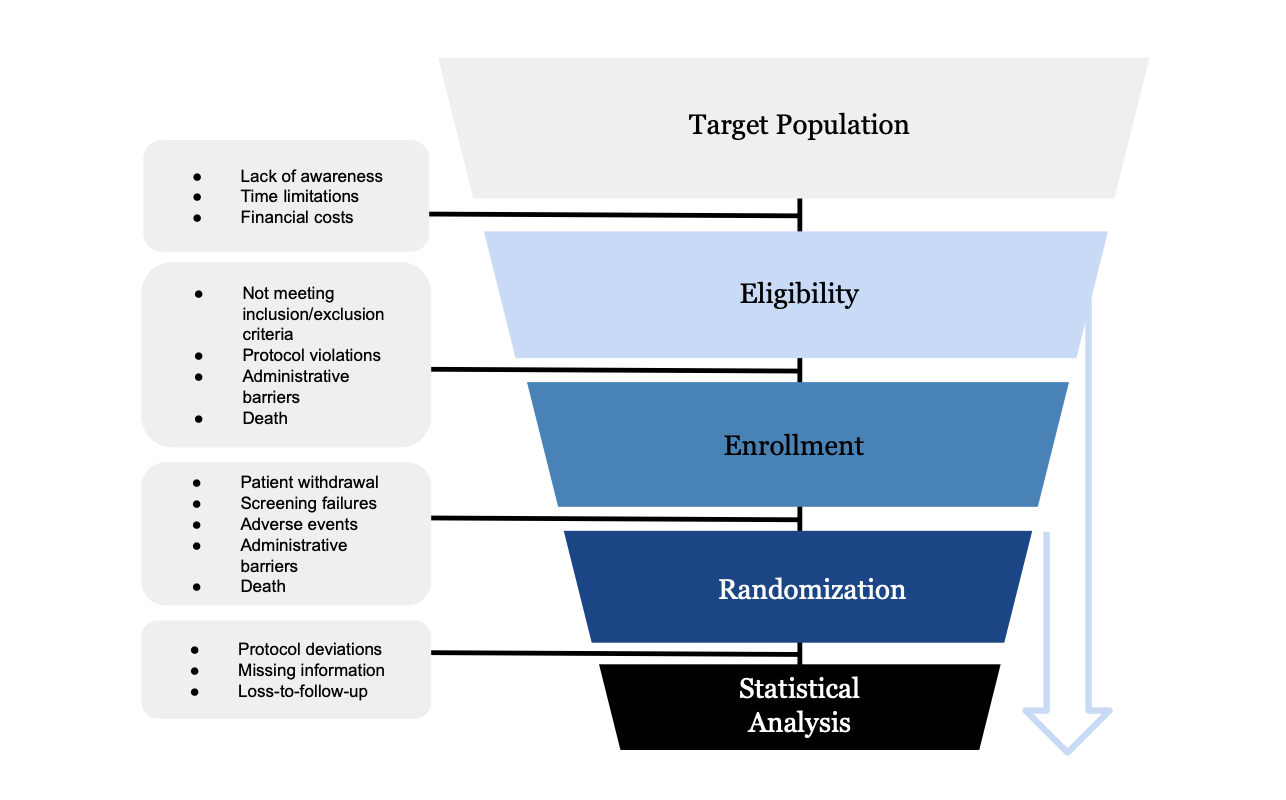
\includegraphics[width=0.7\textwidth]{fig_2_1_a.png}
  \caption{Patient recruitment and leakage at each stage of a clinical study \citep{piantadosi2022principles, whelan2018high, bogin2022lasagna}.}
  \label{fig:2_1_a}
\end{figure}

\begin{figure}[h]
  \centering
  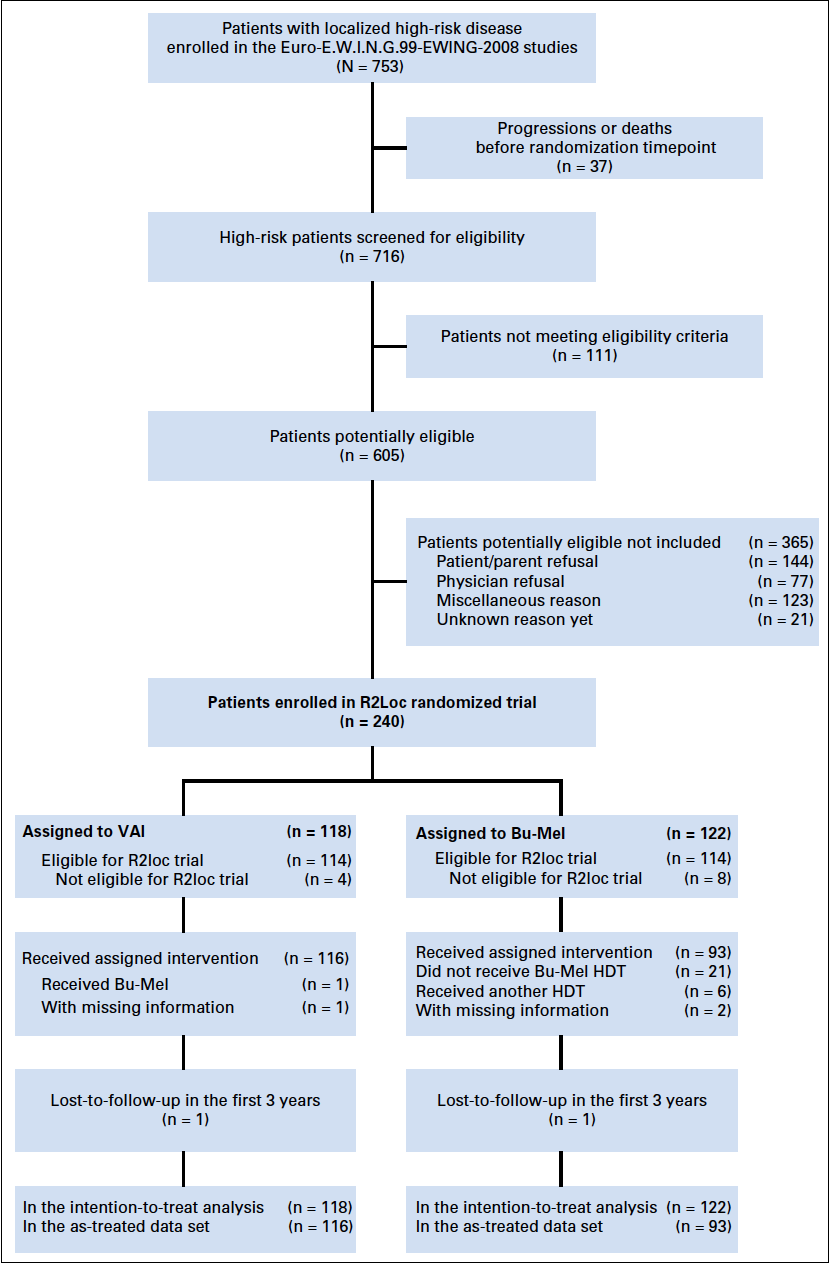
\includegraphics[width=0.7\textwidth]{whelan_flow.png}
  \caption{PRISMA study flow-chart \citep{whelan2018high}.}
  \label{fig:2_0}
\end{figure}

The number of patients decreases at each stage of a clinical study, from defining the target population to final statistical analysis, see Figure \ref{fig:2_1_b}. This process is known as patient leakage \citep{desai2014preventing}, alternative terms are attrition or retention.

Figure \ref{fig:2_1_a} generalizes the notion of patient leakage found in trial profiles such as the one found in Figure \ref{fig:2_0}. Figure \ref{fig:2_1_a} outlines the various stages of a clinical trial and analyzes the key factors contributing to patient attrition as they transition from one stage to the next.

Eligibility criteria narrow down participants, and enrollment further reduces numbers as only those meeting strict criteria are registered. Randomization assigns individuals to treatment groups, but some may later be excluded due to protocol deviations, missing data, or loss to follow-up. 


\begin{figure}[h]
  \centering
  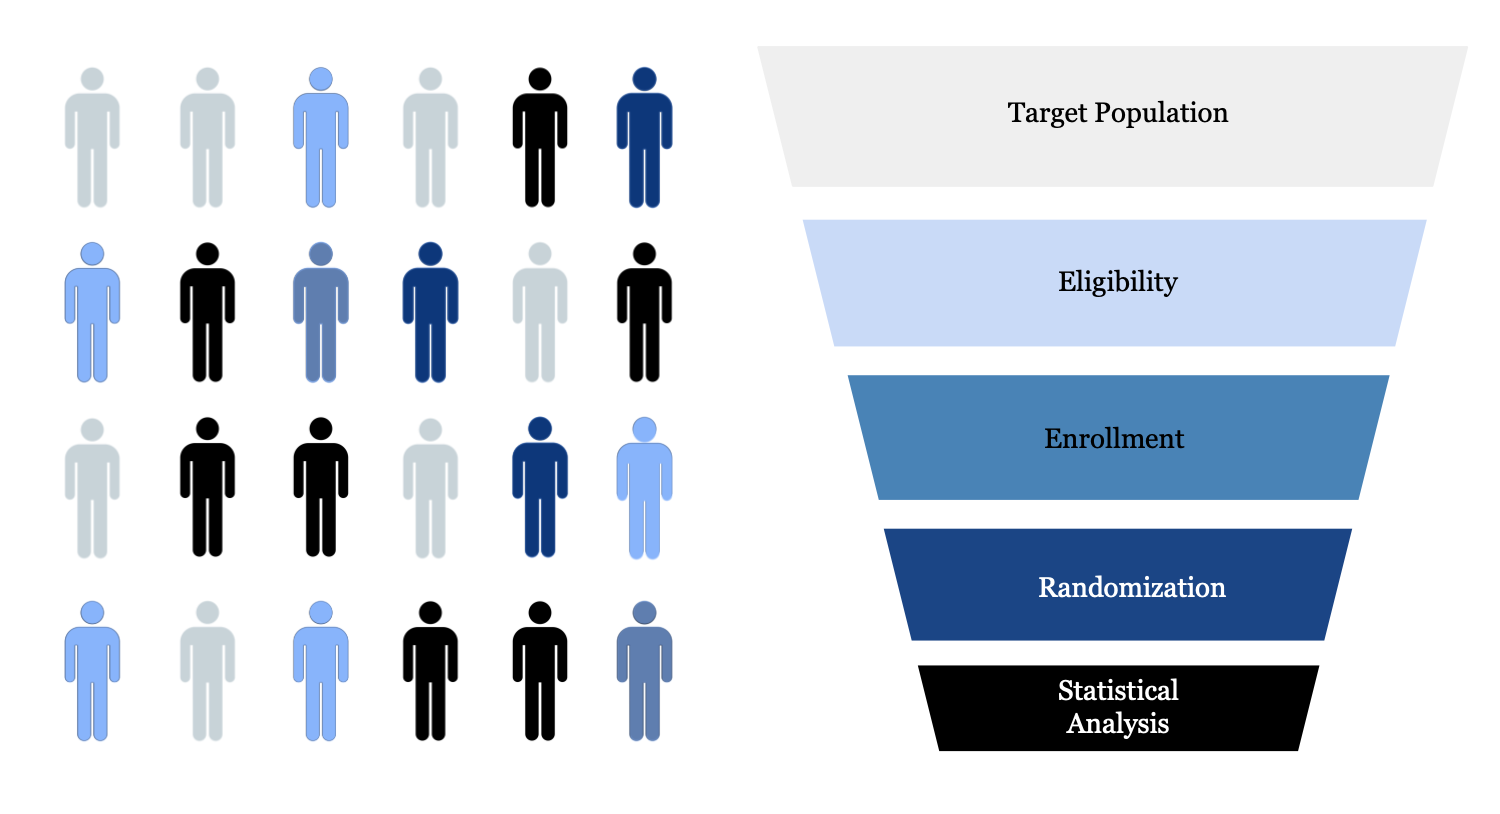
\includegraphics[width=0.7\textwidth]{fig_2_1_b.png}
  \caption{Visual representation of patient recruitment and leakage at each stage of a clinical study \citep{piantadosi2022principles, whelan2018high, bogin2022lasagna}.}
  \label{fig:2_1_b}
\end{figure}

\section{Uncertainty and models for counts and time}

There are two types of uncertainty, aleatory and epistemic \citep{ohagan2006}. The \textbf{Aleatory Uncertainty} reflects randomness that is inherent, irreducible and unpredictable in nature. \textbf{Epistemic Uncertainty} arises primarily from limited or imperfect knowledge about the parameters of a statistical model and can reflect fluctuations of the parameter. Obtaining more or better information about the parameter typically reduces the epistemic uncertainty. 


Let us denote

\begin{itemize}
\item $T=time$
\item $C=counts$
\item $\lambda=\frac{C}{T}$
\end{itemize}

We define \textbf{Recruitment Rate} $\lambda=\frac{C}{T}$ at which patients are collected, measured as persons per unit of time, where \textbf{Rate} is understood as a ratio in which the numerator and denominator are incremental differences \citep{piantadosi2024clinical}:

\begin{align*}
\lambda = \frac{\Delta C}{\Delta T} = \frac{C_1 - C_0}{T_1 - T_0} = \frac{C_1 - 0}{T_1 - 0} = \frac{C_1}{T_1}
\end{align*}


\begin{table}[h!]
\centering
\resizebox{\textwidth}{!}{
\begin{tabular}{cccccc}
 \textbf{Methods} & \textbf{Counts} & \textbf{Expectation} & \textbf{Variance} & \textbf{Aleatory} & \textbf{Epistemic} \\
\hline
\hline
Expectation & $C = \lambda  $ & $\lambda  $ & 0 & No & No \\
Poisson & $C \sim \textrm{Po} (\lambda )$ & $\lambda $ & $\lambda  $ & Yes & No \\
Poisson-Gamma & $C \sim \textrm{Po} (\Lambda )$; $\Lambda \sim \textrm{G}(\alpha,\beta)$ & $\frac{\alpha}{\beta}$ & $\frac{\alpha(\beta+1)}{\beta^2}$ & Yes & Yes \\
\end{tabular}
}
\caption{Moments and aleatory and epistemic uncertainty of recruitment in one unit of time recruitment covered by different models for counts.}
\label{tab:count_modeling}
\end{table}




\begin{table}[h!]
\centering
\resizebox{\textwidth}{!}{
\begin{tabular}{cccccc}
 \textbf{Methods} & \textbf{Counts} & \textbf{Expectation} & \textbf{Variance} & \textbf{Aleatory} & \textbf{Epistemic} \\
\hline
\hline
Expectation & $C(t) = \lambda  t$ & $\lambda  t$ & 0 & No & No \\
Poisson & $C(t) \sim \textrm{Po} (\lambda  t)$ & $\lambda  t$ & $\lambda  t$ & Yes & No \\
Poisson-Gamma & $C(t) \sim \textrm{Po} (\Lambda  t)$; $\Lambda \sim \textrm{G}(\alpha,\beta)$ & $t\frac{\alpha}{\beta}$ & $t\frac{\alpha(\beta+t)}{\beta^2}$ & Yes & Yes \\
\end{tabular}
}
\caption{Moments and aleatory and epistemic uncertainty in accrual until $t$ covered by different models for counts.}
\label{tab:count_modeling_2}
\end{table}


\begin{table}[h!]
\centering
\resizebox{\textwidth}{!}{
\begin{tabular}{cccccc}
 \textbf{Methods} & \textbf{Time} & \textbf{Expectation} & \textbf{Variance} & \textbf{Aleatory} & \textbf{Epistemic} \\
\hline
\hline
Expectation & $T(c) = c/\lambda$ & $c/\lambda$ & 0 & No & No \\
Erlang & $T(c) \sim \textrm{G}(c, \lambda) $ & $c/\lambda$ & $c/\lambda^2$ & Yes & No \\
Gamma-Gamma & $T(c) \sim \textrm{G}(c, \Lambda)$; $\Lambda \sim \textrm{G}(\alpha,\beta)$ & $c\frac{\beta}{\alpha-1}$ & $\frac{c\beta^2(c+\alpha-1)}{(\alpha-1)^2(\alpha-2)}$ & Yes & Yes \\
\end{tabular}
}
\caption{Moments and aleatory and epistemic uncertainty of recruitment covered by different models for time having a fixed sample size $c$.}
\label{tab:time_modeling}
\end{table}


Methods in Tables \ref{tab:count_modeling}, \ref{tab:count_modeling_2} and \ref{tab:time_modeling} are applicable to each level of recruitment in Figures \ref{fig:2_1_a} and \ref{fig:2_1_b}.

\chapter{Methods for Counts} 
\section{Counts: Model based on Expectations}
\label{sec:expect}

If we fix the duration of a study at time $T$ and we expect that we collect $C$ patients until $T$, we deterministically predict the recruitment rate per one unit of time (without taking into consideration any uncertainty) to be $\hat{\lambda}=\frac{C}{T}$ \citep{carter2004application}. Researchers tend to use simple unconditional methods \citep{white2015projection}.




\subsection{Expected recruitment in one unit of time}
$C = \textrm{E}C = \textrm{E}\lambda = \lambda$\\
$\textrm{Var}(C) = \textrm{Var}(\lambda) = 0$

As we can see in Table \ref{tab:count_modeling}

\subsection{Expected accrual at time point $t$}

Assuming that recruitments in each unit of time are independent of each other we have:

$C(t) = \textrm{E}(\underbrace{C+\ldots+C}_{t \ \text{times}}) = \textrm{E}(\lambda t) = \lambda t$\\
$\textrm{Var}(C(t)) = \textrm{Var}(\underbrace{C+\ldots+C}_{t \ \text{times}}) = t \textrm{Var}(\lambda) = 0$

Both the expected accrual and its zero-variance are recorded in Table \ref{tab:count_modeling_2}
and visualized in Figure \ref{fig:2_2} and Figure \ref{fig:2_5}.

\subsection{Criticism}

This is a simple deterministic method based on a linear extrapolation of the constant expected recruitment also called "First Order Recruitment Model" (FORM) \citep{comfort2013}. It is also referred to as the \textit{unconditional approach} and its main limitation is the lack of a mechanism to account for known sources of variation in the rate \citep{carter2005practical}. 

The model based on expectations is overly simplistic and fails to account for changes in center recruitment or the regulatory environment \citep{barnard2010systematic}. Therefore, stochastic models that incorporate randomness in the recruitment process are more suitable than the widely used deterministic approach \citep{zhang2012modeling}.

\section{Counts: Model based on Poisson Process}

One way to incorporate variation in the mean number of participants per day is by assuming that participants are recruited according to a known probability distribution, such as the Poisson distribution \citep{carter2004application}. This approach emulates trial accrual using a random number generator and records the time required to reach the target sample size over multiple iterations \citep{carter2005practical}. 

The resulting distribution helps estimate the probability of completing accrual within a given time frame and assess variability in accrual time. This method is particularly useful when a trial has a fixed duration, as it allows researchers to determine the necessary number of clinical centers and monthly recruitment rate to achieve a high probability (e.g., 80\%) of completing enrollment on time \citep{carter2005practical}.

The Poisson distribution $C\sim \rm{Po} (\lambda)$ allows us to explain the recruitment of patients. It is a discrete variable that expresses the probability of a given number of events (in our case, patient recruitment) occurring in a fixed unit interval of time. We assume that these events occur with a known constant rate $\lambda$ and are independent of each other.

\begin{align*}
\textrm{P}[C=&c] = \frac{\lambda^c}{c!}e^{-\lambda} \\
&c = 0,1,2,\ldots
\end{align*}


One important property from the Poisson distribution is that it is infinitely divisible \citep{held2014applied}. If $X_i\sim \textrm{Po} (\lambda_i)$ for $i=1,\ldots, n$ are independent, then, $\sum_{i=1}^n X_i \sim \textrm{Po} \Big( \sum_{i=1}^n \lambda_i \Big)$.

\subsection{Recruitment in one unit of time}

The recruitment of patients in one unit of time follows $C\sim \textrm{Po} (\lambda)$ and the expectation and variance are:

\begin{align*}
\textrm{E}C & = \lambda \\
\textrm{Var}(C) & = \lambda
\end{align*}

As we can see in Table \ref{tab:count_modeling}

\subsection{Accrual at time point $t$}
At time point $t$, the accrual follows $C\sim \textrm{Po} (\lambda t)$. Using the infinitely divisible property from the Poisson applicable to independent random variables, $\underbrace{\textrm{Po} (\lambda) +\cdots +\textrm{Po} (\lambda)}_{t \ \text{times}} = \textrm{Po} (\lambda t)$. We assume that the recruitment of patients in $t$ unit time intervals is independent from another. As we can see in Table \ref{tab:count_modeling_2}, the expectation and variance are the following:

\begin{align*}
\textrm{E}C(t) & = \lambda t \\
\textrm{Var}(C(t)) & = \lambda t
\end{align*}

For example, if we assume $\lambda = 0.591$ per day and $t=550$, we can show the accrual of 100 different studies in Figure \ref{fig:2_2} and the histogram at $t=550$ days. The exact distribution at $t=550$ is provided in Figure \ref{fig:2_3} and the Cummulative Distribution Function (CDF) in Figure \ref{fig:2_4}. The uncertainty bands based on the exact quantiles are displayed in Figure \ref{fig:2_5}.

\begin{figure}
\begin{knitrout}
\definecolor{shadecolor}{rgb}{0.98, 0.98, 0.98}\color{fgcolor}

{\centering 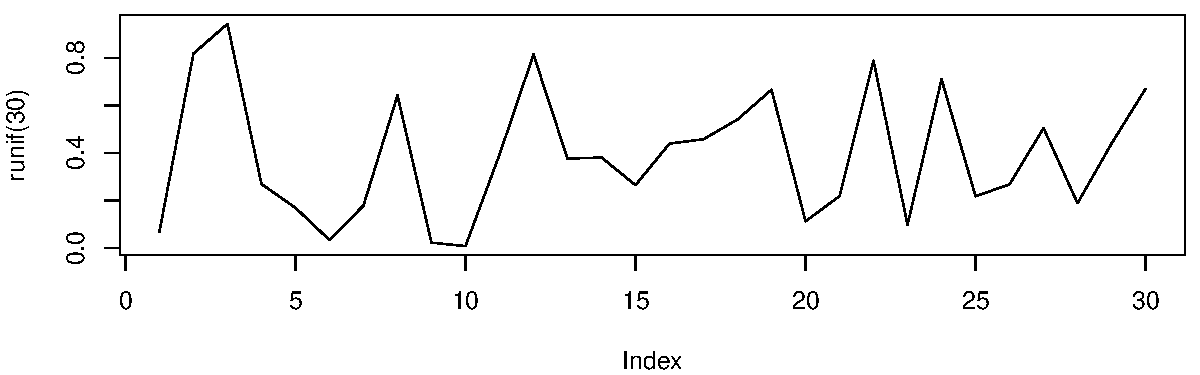
\includegraphics[width=\textwidth-3cm]{figure/ch02_figunnamed-chunk-3-1} 

}


\end{knitrout}
  \caption{Poisson-distributed counts with $\lambda = 0.591$ per day and uncertainty range. The black line represents the point estimate of the expected accrual from section \ref{sec:expect}, while the red dashed lines indicate Poisson's 95\% aleatory uncertainty. The histogram illustrates the distribution of observed counts in 100 studies at time $t = 550$ days \citep{spiegelhalter2011visualizing, pkgacc}.}
  \label{fig:2_2}
\end{figure}


\begin{figure}
\begin{knitrout}
\definecolor{shadecolor}{rgb}{0.98, 0.98, 0.98}\color{fgcolor}

{\centering 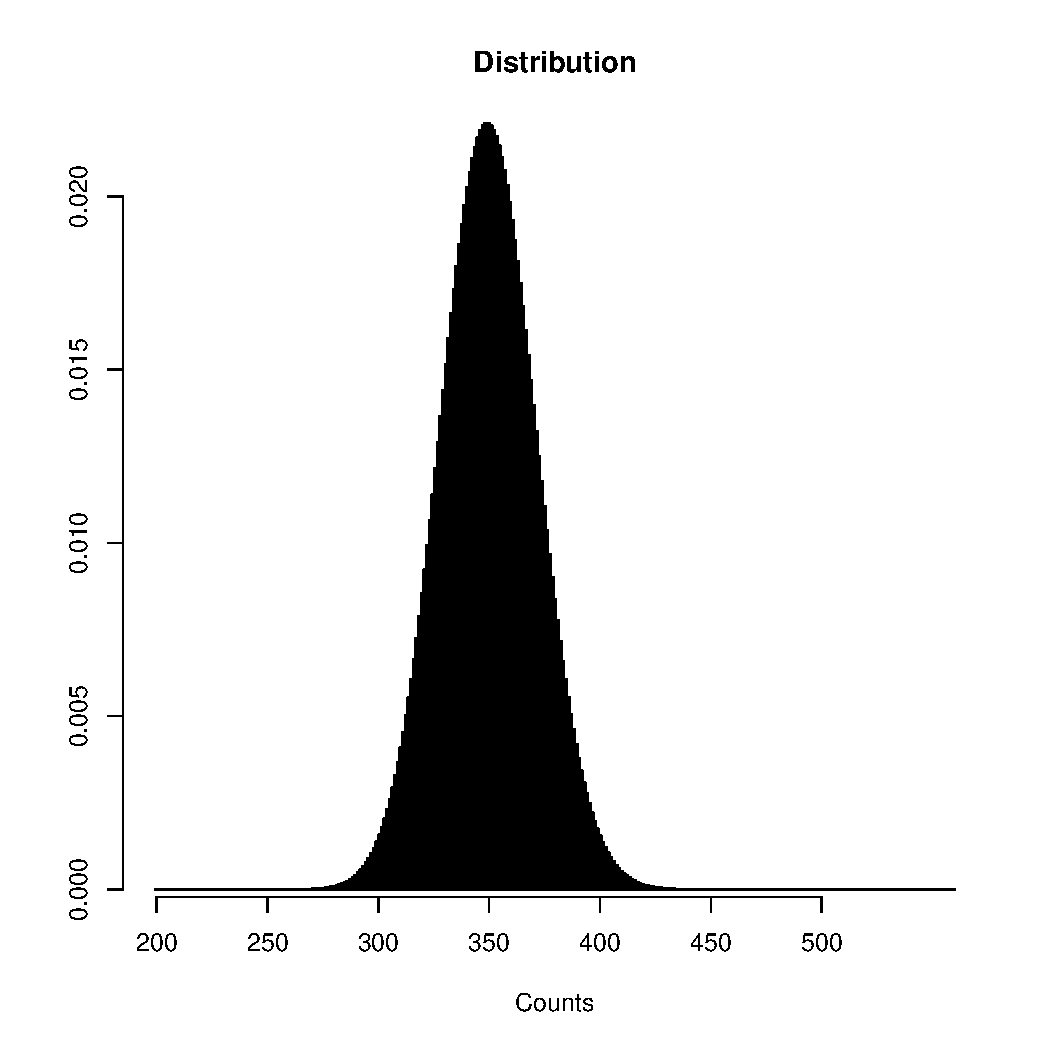
\includegraphics[width=\textwidth-3cm]{figure/ch02_figunnamed-chunk-4-1} 

}


\end{knitrout}
  \caption{Probability Mass Function (PMF) of Poisson-distributed counts: This bar plot represents the probability mass function (PMF) of counts ranging from 200 to 500, using a Poisson distribution $\textrm{Po}(\lambda t)$ with a rate parameter $\lambda = 0.591$ per day at time $t = 550$ days.}
  \label{fig:2_3}
\end{figure}

\begin{figure}
\begin{knitrout}
\definecolor{shadecolor}{rgb}{0.98, 0.98, 0.98}\color{fgcolor}

{\centering 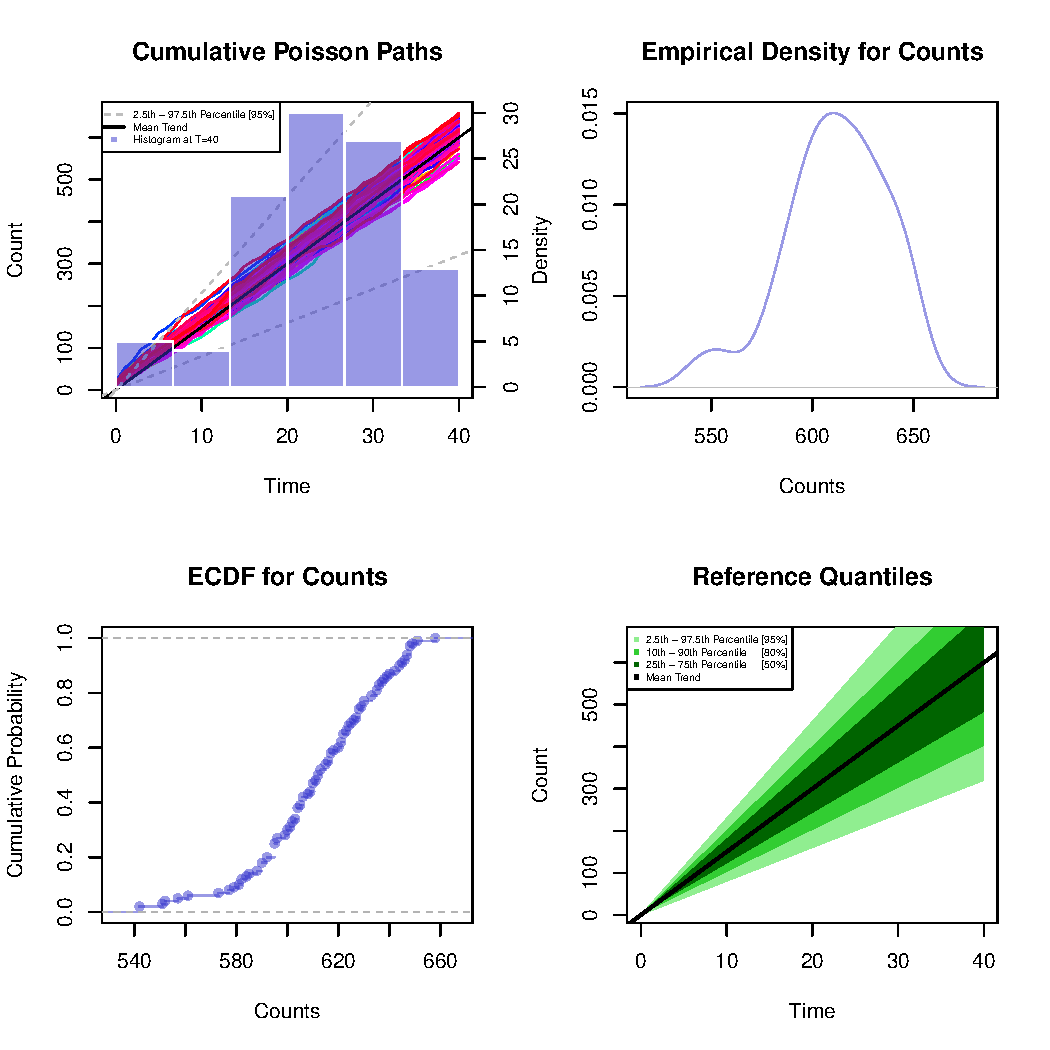
\includegraphics[width=\textwidth-3cm]{figure/ch02_figunnamed-chunk-5-1} 

}


\end{knitrout}
  \caption{Cumulative Distribution Function (CDF) of Poisson-distributed counts: The bar plot illustrates the cumulative probability distribution for counts within the range of 200 to 500, using a Poisson $\textrm{Po}(\lambda t)$ distribution with a rate parameter $\lambda = 0.591$ per day at time $t=550$ days.}
  \label{fig:2_4}
\end{figure}


\begin{figure}
\begin{knitrout}
\definecolor{shadecolor}{rgb}{0.98, 0.98, 0.98}\color{fgcolor}

{\centering 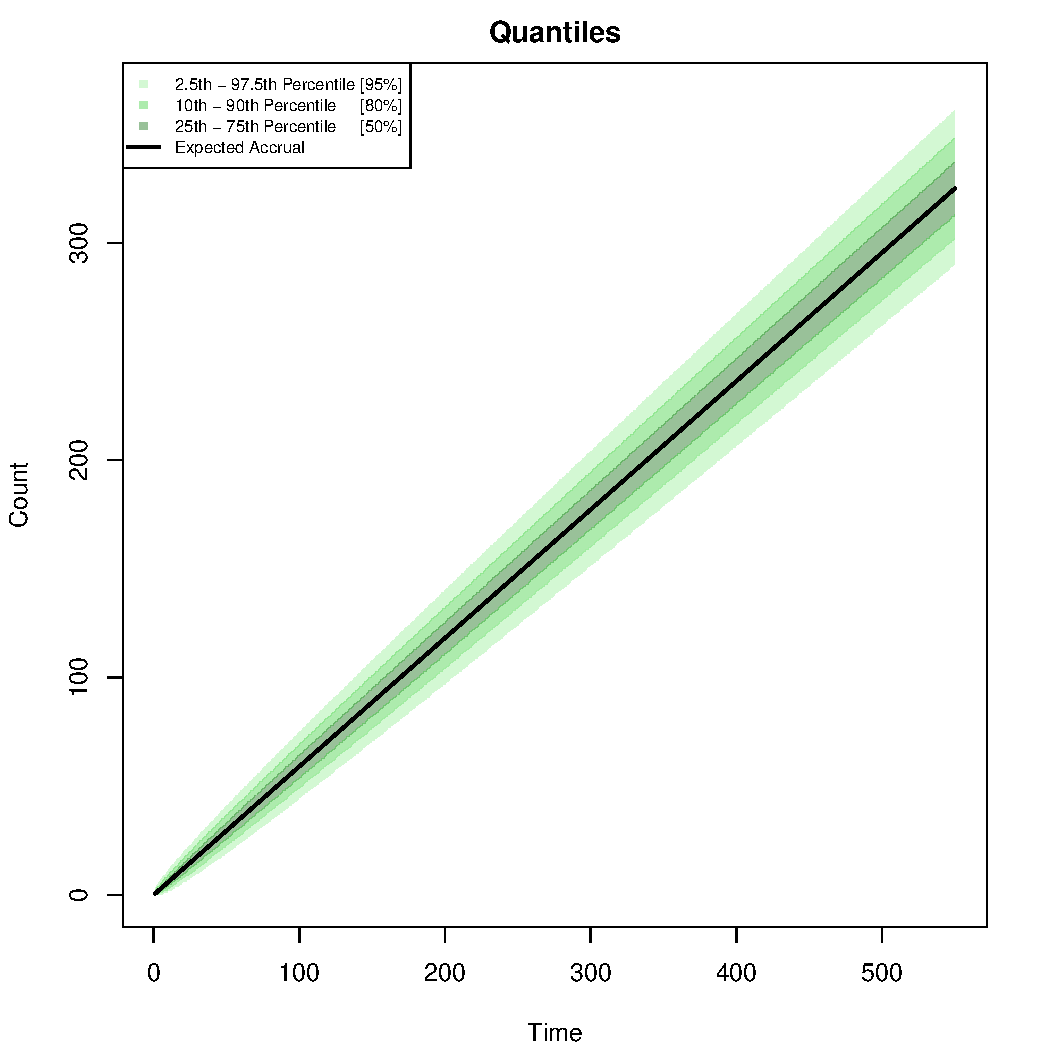
\includegraphics[width=\textwidth-3cm]{figure/ch02_figunnamed-chunk-6-1} 

}


\end{knitrout}
  \caption{Predicted uncertainty bands for Poisson process with $\lambda = 0.591$ per day. The black line represents the expected accrual, while the red shaded regions indicate aleatory uncertainty: the dark red band spans the interquantile range (25th - 75th percentiles), the lighter red band cover the 10th - 90th percentile range and the light red the 2.5th - 97.5th percentile range \citep{spiegelhalter2011visualizing}.}
  \label{fig:2_5}
\end{figure}

\subsection{Criticism}

This model was used by \cite{carter2004application} and \cite{carter2005practical}. Although this model accounts for aleatory uncertainty, the recruitment rate is assumed to be constant for the entire period of time. Therefore, an alternative method that accounts for varying recruitment rates over time is necessary.

\section{Counts: Negative Binomial model derived from Poisson-Gamma model}

The basic Poisson model does not account for variations in recruitment rates or uncertainties in rate estimates \citep{mountain2022recruitment}. To address this \cite{anisimov2007modelling} propose a random effects model where recruitment follows a homogeneous Poisson process with rates drawn from a gamma distribution, a probabilistic model with Poisson-Gamma mixture distribution. In this approach, rates are treated as random variables with a prior gamma distribution, whose parameters are estimated using current recruitment data. This allows for a posterior distribution of rates to be used for recruitment prediction in an empirical Bayesian framework.  

Building on this, a Poisson-Gamma model can be implemented by randomly generating recruitment rates using a Gamma distribution and plugging them into a Poisson process. This model can be used to make two types of projections: a point prediction estimating when the expected number of events will reach a specific sample size and a Bayesian interval prediction based on the generation of future accrual and event dates. This method enables flexible forecasting for any milestone at any calendar time \citep{bagiella2001predicting}.


\begin{figure}
\begin{knitrout}
\definecolor{shadecolor}{rgb}{0.98, 0.98, 0.98}\color{fgcolor}

{\centering 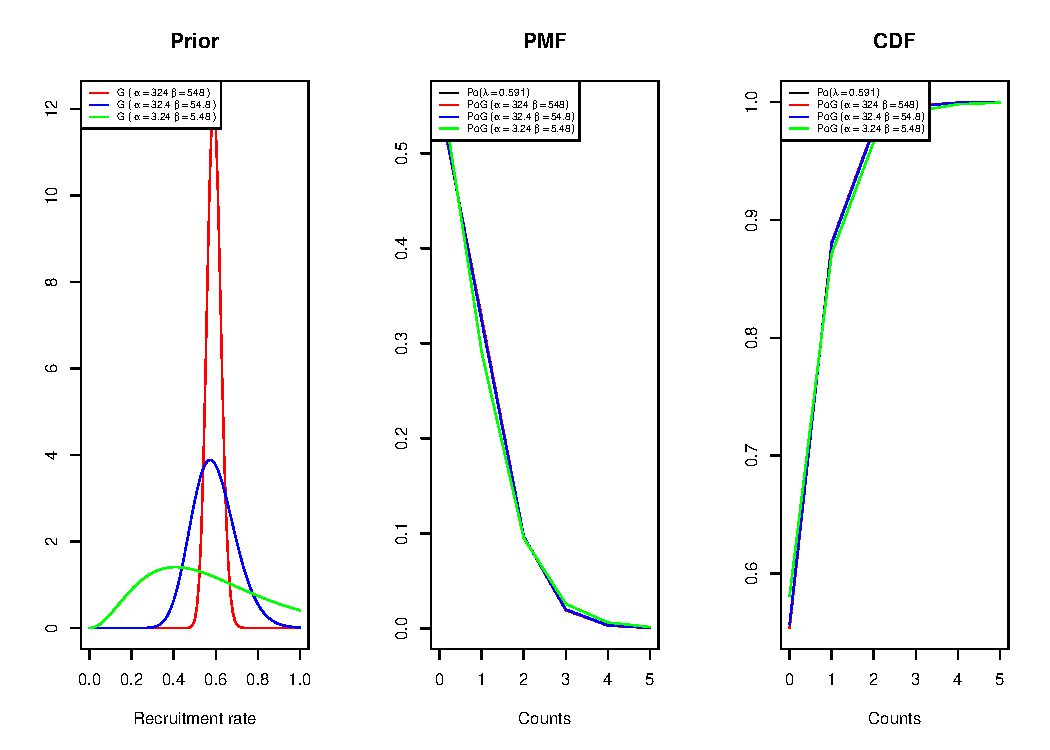
\includegraphics[width=\textwidth-3cm]{figure/ch02_figunnamed-chunk-7-1} 

}


\end{knitrout}
	\caption{Sensitivity analysis between Poisson distribution with $\lambda = 0.591$ and Negative Binomial changing parameters of Gamma prior that maintain same expectation $\frac{\alpha}{\beta} = 0.591$ with $t=1$.}
  \label{fig:2_6}
\end{figure}

\subsection{Recruitment in one unit of time}

Let $C|\Lambda \sim \textrm{Po}(\Lambda)$ and $\Lambda \sim \textrm{G}(\alpha,\beta)$. Where $\Lambda$ represents the "recruitment proneness" in the unit of time. 

\begin{align*}
p(c)&=\int^\infty_0 p(c|\lambda) p(\lambda) d\lambda\\
&=\int^\infty_0 \frac{\lambda^c\exp(-\lambda)}{c!}\Bigg[\lambda^{\alpha-1}\exp(-\beta\lambda)\frac{\beta^\alpha}{\Gamma(\alpha)}\Bigg]d\lambda\\
&=\frac{\beta^\alpha}{c!\Gamma(\alpha)}\int^\infty_0 \lambda^{\alpha+c-1}\exp(-\lambda)\exp(-\lambda\beta)d\lambda\\
&=\frac{\beta^\alpha\Gamma(\alpha+c)}{c!\Gamma(\alpha) (\beta+1)^{\alpha+c}}\underbrace{\int^\infty_0 \frac{(\beta+1)^{\alpha+c}}{\Gamma(\alpha+c)} \lambda^{\alpha+c-1}\exp(-(\beta+1)\lambda)d\lambda}_{=1}\\
&=\beta^\alpha\binom{\alpha+c-1}{\alpha-1}\Bigg (\frac{1}{\beta+1}\Bigg)^{\alpha+c}\\
&=\binom{\alpha+c-1}{\alpha-1}\Bigg (\frac{1}{\beta+1}\Bigg)^{c} \Bigg(\frac{\beta}{\beta+1}\Bigg)^{\alpha}\\
& c = 0,1,2,3,\ldots
\end{align*}

Thus, $C\sim \textrm{NBin} \Bigg(\alpha, \frac{\beta}{\beta+1}\Bigg)$.


The parameter $\lambda$ in the integral represents the expected recruitment rate per unit of time for an individual and this recruitment rate is assumed to vary from individual to individual as it is generated by a $\textrm{G}(\alpha,\beta)$ distribution \citep{johnson2005univariate}.


Using the expressions of iterated expectation and variance \citep{held2014applied} and the expectation and variance from the respective random variables $C|\Lambda \sim \textrm{Po}(\Lambda)$ and $\Lambda \sim \textrm{G}(\alpha,\beta)$, we have that:


\begin{align*}
\textrm{E}C &= \textrm{E}_{\Lambda}[\textrm{E}_{C} (C|\Lambda)] = \textrm{E}_{\Lambda}[\Lambda] = \alpha/\beta
\end{align*}

\begin{align*}
\textrm{Var}(C) &= \textrm{Var}_{\Lambda}[\textrm{E}_{C} (C|\Lambda)] + \textrm{E}_{\Lambda}[\textrm{Var}_C(C|\Lambda)]\\
&=\textrm{Var}_{\Lambda}[\Lambda] + \textrm{E}_{\Lambda}[\Lambda] \\
&=\alpha/\beta^2 + \alpha/\beta = \frac{\alpha(\beta+1)}{\beta^2}
\end{align*}


There are two different interpretations of the Negative Binomial, Failure-Based and Count-based.
\subsection{Failure-Based}
\begin{enumerate}
\item The Negative Binomial $X\sim\textrm{NBin}(r,\pi)$ models the number of \textbf{failures} before achieving a fixed number of \textbf{successes} in a sequence of Bernoulli trials. 
\item Parametrization:
	\begin{itemize}
	\item $n$: Number of successes to be achieved (fixed).
	\item $p$: Probability of success in each trial
	\item The random variable $X$ represents the number of failures before achieving $n$ successes.
	\end{itemize}
\item Probability Mass Function (PMF) \citep{R-stats}:
\begin{align*}
\textrm{P}(X=&x) = \frac{\Gamma(x+n)}{\Gamma(x) x!}  p^n(1-p)^x, \\
&x = 0,1,2, \ldots, n >0\\
&0<p\leq 1
\end{align*}
where $x$ is the number of failures.
\item Interpretation: In a sequence of independent binary trials with constant probability $p$ of observing a \textit{non-recruited} patient, $X$ is the number of \textit{recruited} patients observed at the time that $x$ \textit{non-recruited} patients are observed \citep{meeker2017statistical}.


\end{enumerate}

With respect to the parameters, $n>0$ represents the number of successes until 
the experiment is stopped. The success probability in each experiment is 
represented by $p\in[0,1]$.  In R the functions \_\texttt{nbinom(..., size = $n$, prob = $p$)} relate to the random variable $X-r$, the number of successes (as opposed to the number of trials) until $r$ successes have been achieved \citep{held2014applied}. 

\begin{align*}
EX & = \frac{r(1-\pi)}{\pi}\\
Var(X) & = \frac{r(1-\pi)}{\pi^2}
\end{align*}

Since we will be using the Count-Based interpretation of the Negative Binomial \citep{hilbe2011negative}, our parametrization relates to R with $n = \alpha$ and $p = \frac{\beta}{\beta+1}$.

\subsection{Count-Based}
\begin{enumerate}
\item The Negative Binomial $X\sim\textrm{NBin}\Bigg(\alpha,\frac{\beta}{\beta+1}\Bigg)$ can also be seen as a Poisson-Gamma mixture, where the observed count data follows a Poisson distribution with a mean that itself follows a Gamma distribution, $C|\Lambda \sim \textrm{Po}(\Lambda)$ and $\Lambda \sim \textrm{G}(\alpha,\beta)$. 
\item Parametrization:
	\begin{itemize}
	\item $\mu = \frac{\alpha}{\beta}$: Mean of the distribution (expected number of occurrences).
	\item $\alpha$: Dispersion parameter, controlling the variance.
	\end{itemize}
\item Alternative formulation of the PMF \citep{hilbe2011negative}:
\begin{align*}
\textrm{P}(X=&c) = \binom{\alpha+c-1}{\alpha-1}\Bigg (\frac{\mu}{\beta+\mu}\Bigg)^{c} \Bigg(\frac{\alpha}{\alpha+\mu}\Bigg)^{\alpha}, \\
&c\geq 0 
\end{align*}
where $c$ is the counts.
\item Interpretation: This model is used to represent "recruitment proneness". The parameter $\mu$ represents the expected number of recruitments in a study \citep{johnson2005univariate}.

\end{enumerate}

In the count-based method we take into account the overdispersion of the data. When the variability in the observed data is greater than what is expected.

\begin{align*}
\textrm{E}X&=\mu\\
\textrm{Var}X&=\mu + \frac{\mu}{\beta}
\end{align*}

How do we get to our formulation of the PMF:

\begin{align*}
\textrm{P}(X=c) & = \binom{\alpha+c-1}{\alpha-1}\Bigg (\frac{\mu}{\alpha+\mu}\Bigg)^{c} \Bigg(\frac{\alpha}{\alpha+\mu}\Bigg)^{\alpha} \\
& = \binom{\alpha+c-1}{\alpha-1}\Bigg (\frac{\alpha/\beta}{\alpha+\alpha/\beta}\Bigg)^{c} \Bigg(\frac{\alpha}{\alpha+\alpha/\beta}\Bigg)^{\alpha} \\
& = \binom{\alpha+c-1}{\alpha-1}\Bigg (\frac{\alpha/\beta}{\alpha\beta/\beta+\alpha/\beta}\Bigg)^{c} \Bigg(\frac{\alpha}{\alpha\beta/\beta+\alpha/\beta}\Bigg)^{\alpha} \\
& = \binom{\alpha+c-1}{\alpha-1}\Bigg (\frac{\alpha}{\alpha\beta+\alpha}\Bigg)^{c} \Bigg(\frac{\beta\alpha}{\alpha\beta+\alpha}\Bigg)^{\alpha} \\
&= \binom{\alpha+c-1}{\alpha-1}\Bigg (\frac{1}{\beta+1}\Bigg)^{c} \Bigg(\frac{\beta}{\beta+1}\Bigg)^{\alpha}
\end{align*}



% 
% \begin{align*}
% Mean &= \frac{\alpha\bigg(1-\frac{\beta}{\beta+1}\bigg)}{\frac{\beta}{\beta+1}}\\
% &= \frac{\alpha\bigg (\frac{1}{\beta+1}\bigg)}{\frac{\beta}{\beta+1}}\\
% &= \frac{\alpha(\beta+1)}{\beta(\beta+1)}\\
% &= \frac{\alpha}{\beta}
% \end{align*}
% 
% \begin{align*}
% Variance &= \frac{\alpha\bigg(1-\frac{\beta}{\beta+1}\bigg)}{\bigg(\frac{\beta}{\beta+1}\bigg)^2}\\
% &= \frac{\alpha\bigg (\frac{1}{\beta+1}\bigg)}{\bigg(\frac{\beta}{\beta+1}\bigg)^2}\\
% &= \frac{\alpha(\beta+1)^2}{\beta^2(\beta+1)}\\
% &= \frac{\alpha(\beta+1)}{\beta^2}
% \end{align*}


\begin{figure}
\begin{knitrout}
\definecolor{shadecolor}{rgb}{0.98, 0.98, 0.98}\color{fgcolor}

{\centering 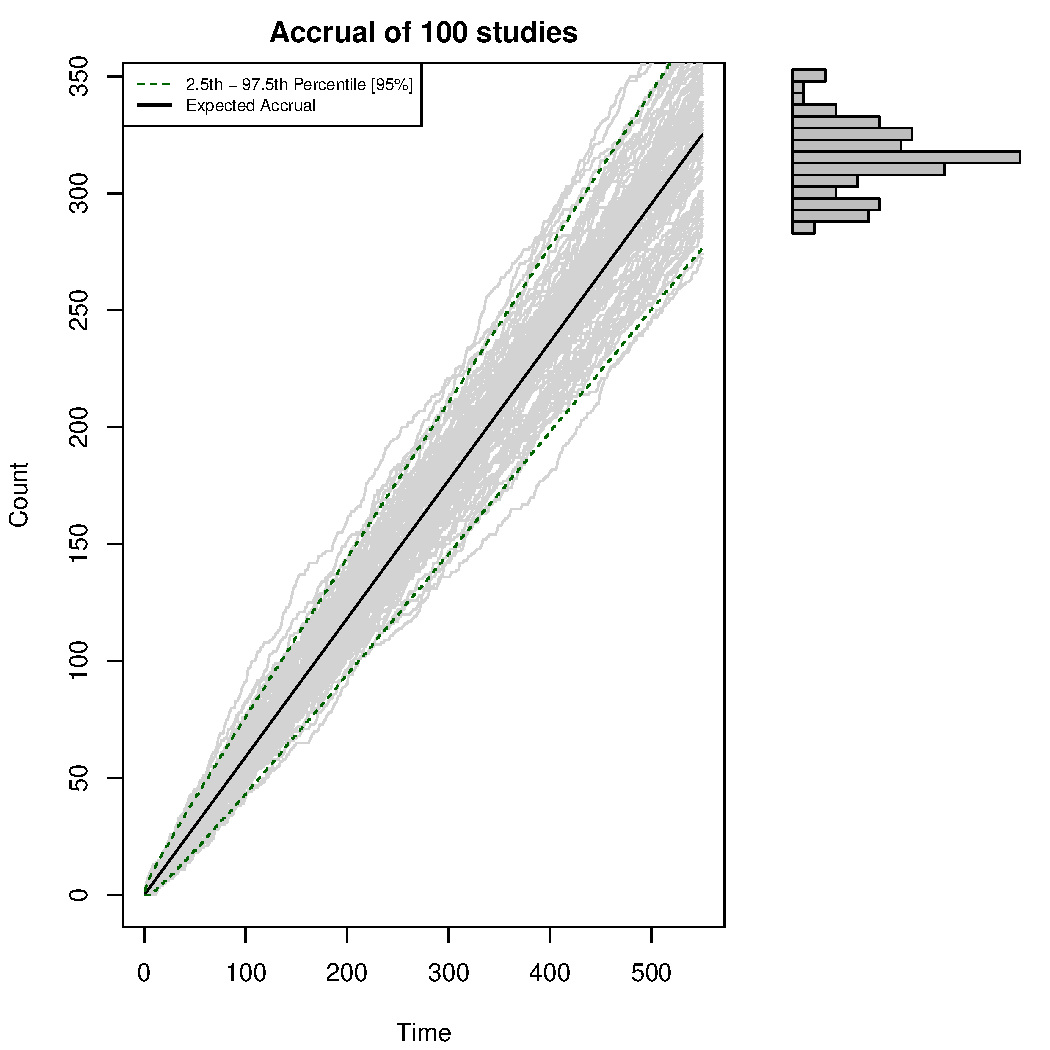
\includegraphics[width=\textwidth-3cm]{figure/ch02_figunnamed-chunk-8-1} 

}


\end{knitrout}
  \caption{Poisson-Gamma $(\alpha = 324, \beta = 548)$ distributed counts with $\mu = 0.591$ per day and uncertainty range. The black line represents the point estimate of the expected accrual from Section \ref{sec:expect}, while the red dashed lines indicate Poisson-Gamma 95\% aleatory and epistemic uncertainty. The histogram illustrates the distribution of observed counts in 100 studies at time $t = 550$ days \citep{spiegelhalter2011visualizing, pkgacc}.}
  \label{fig:2_7}
\end{figure}



\begin{figure}
\begin{knitrout}
\definecolor{shadecolor}{rgb}{0.98, 0.98, 0.98}\color{fgcolor}

{\centering 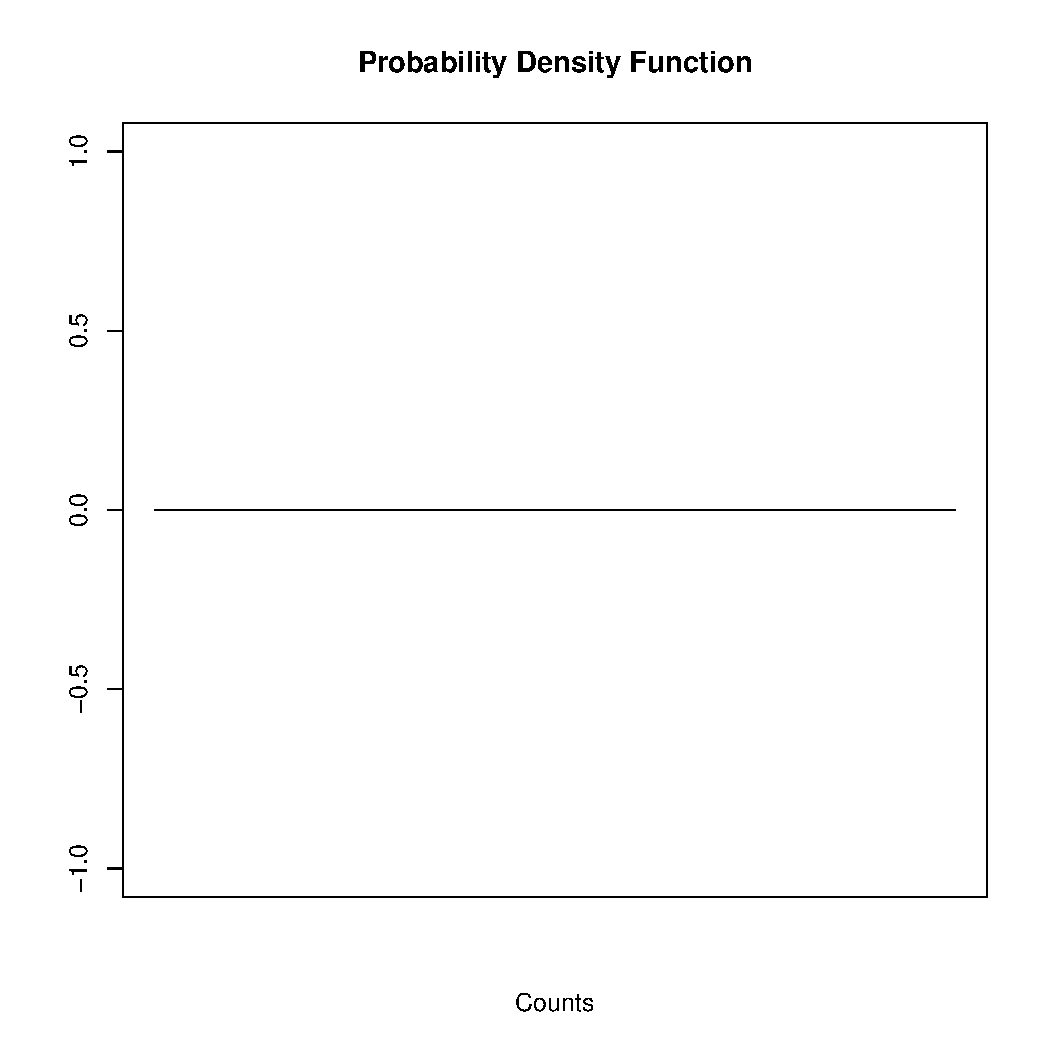
\includegraphics[width=\textwidth-3cm]{figure/ch02_figunnamed-chunk-9-1} 

}


\end{knitrout}
  \caption{Predicted uncertainty bands for Poisson-Gamma process with $\mu = 0.591$ per day. The black line represents the expected accrual, while the green shaded regions indicate aleatory and epistemic uncertainty: the dark green band spans the interquantile range (25th - 75th percentiles), the lighter green band cover the 10th - 90th percentile range and the light green the 2.5th - 97.5th percentile range \citep{spiegelhalter2011visualizing}.}
  \label{fig:2_8}
\end{figure}

\subsection{Sensitivity Analysis}

In Figures \ref{fig:2_6b} and \ref{fig:2_6}, the Poisson distribution captures aleatory uncertainty, while the Gamma prior represents epistemic uncertainty. The Poisson-Gamma distribution incorporates both types of uncertainty. The sensitivity analysis, also shown in Figures \ref{fig:2_6b} and \ref{fig:2_6}, highlights that while the expectation remains unchanged, smaller parameter values lead to greater overall uncertainty due to the increased variance introduced by the Gamma distribution. The smaller the $\beta$, the greater the variance.


\begin{align*}
\textrm{Var}(\textrm{G}(\alpha, \beta)) = \frac{\alpha}{\beta^2} =\frac{\textrm{E}(\textrm{G}(\alpha, \beta))}{\beta}
\end{align*}

In the Poisson-Gamma model we can interpret $\alpha$ as the parameter that represents the sample size and $\beta$ represents time.

\begin{figure}
\begin{knitrout}
\definecolor{shadecolor}{rgb}{0.98, 0.98, 0.98}\color{fgcolor}

{\centering 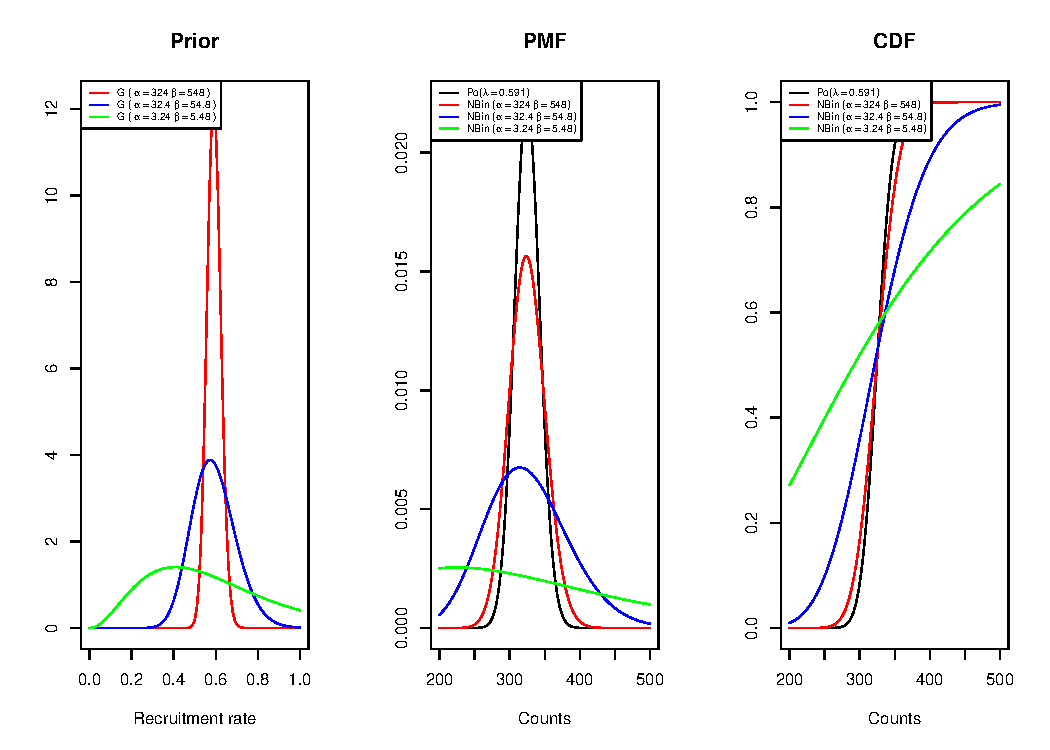
\includegraphics[width=\textwidth-3cm]{figure/ch02_figunnamed-chunk-10-1} 

}


\end{knitrout}
	\caption{Sensitivity analysis between Poisson distribution with $\lambda = 0.591$ and Poisson-Gamma changing parameters of Gamma prior that maintain same expectation $\frac{\alpha}{\beta} = 0.591$ with $t=550$.}
  \label{fig:2_6b}
\end{figure}

\subsection{Accrual at time point $t$}
Let $C(t)|\Lambda \sim \textrm{Po}(\Lambda t)$ and $\Lambda \sim \textrm{G}(\alpha,\beta)$. By the infinitely divisible property of the Poisson distribution we have that $\underbrace{\textrm{Po} (\Lambda) +\cdots +\textrm{Po} (\Lambda)}_{t \ \text{times}} = \textrm{Po} (\Lambda t)$. 

\begin{align*}
p(c)&=\int^\infty_0 p(c|\lambda t) p(\lambda) d\lambda\\
&=\int^\infty_0 \frac{(\lambda t)^c\exp(-\lambda t)}{c!}\Bigg[(\lambda)^{\alpha-1}\exp(-\beta\lambda )\frac{\beta^\alpha}{\Gamma(\alpha)}\Bigg]d\lambda\\
&=\frac{\beta^\alpha t^c}{c!\Gamma(\alpha)}\int^\infty_0 \lambda^{\alpha+c-1}\exp(-\lambda t)\exp(-\lambda\beta)d\lambda\\
&=\frac{\beta^\alpha\Gamma(\alpha+c) t^c}{c!\Gamma(\alpha) (\beta+t)^{\alpha+c}}\underbrace{\int^\infty_0 \frac{(\beta+t)^{\alpha+c}}{\Gamma(\alpha+c)} \lambda^{\alpha+c-1}\exp(-(\beta+t)\lambda)d\lambda}_{=1}\\
&=\beta^\alpha t^c\binom{\alpha+c-1}{\alpha-1}\Bigg (\frac{1}{\beta+t}\Bigg)^{\alpha+c}\\
&=\binom{\alpha+c-1}{\alpha-1}\Bigg (\frac{t}{\beta+t}\Bigg)^{c} \Bigg(\frac{\beta}{\beta+t}\Bigg)^{\alpha}\\
& c = 0,1,2,3,\ldots
\end{align*}
Thus, $C(t)\sim \textrm{NBin} \Bigg(\alpha, \frac{\beta}{\beta+t}\Bigg)$

We will be focusing on the count-based interpretation of the Negative Binomial distribution. We can relate this interpretation to the more popular failure-based interpretation by seeing $\alpha$ as $n$, the number of successes. In our case, the number of patients we wish to recruit. And, $p = \frac{\beta}{\beta+1}$ which is the probability of success, as the probability of recruiting.


Using the expressions of iterated expectation and variance \citep{held2014applied} and the expectation and variance from the respective random variables $C(t)|\Lambda \sim \textrm{Po}(\Lambda t)$ and $\Lambda \sim \textrm{G}(\alpha,\beta)$, we have that:


\begin{align*}
\textrm{E}(C(t)) &= \textrm{E}_{\Lambda}[\textrm{E}_{C(t)} (C(t)|\Lambda)] = \textrm{E}_{\Lambda}[\Lambda t] = t\alpha/\beta
\end{align*}

\begin{align*}
\textrm{Var}(C(t)) &= \textrm{Var}_{\Lambda}[\textrm{E}_{C(t)} (C(t)|\Lambda)] + \textrm{E}_{\Lambda}[\textrm{Var}_{C(t)}(C(t)|\Lambda)]\\
&=\textrm{Var}_{\Lambda}[\Lambda t] + \textrm{E}_{\Lambda}[\Lambda t] \\
&=t^2\alpha/\beta^2 + t\alpha/\beta = \frac{t\alpha(\beta+t)}{\beta^2}
\end{align*}

Therefore, we clearly have overdispersion $\textrm{Var}(C(t))>\textrm{E}(C(t))$. This can be easily seen because:

\begin{align*}
\textrm{Var}(C(t)) &=\textrm{E}(C(t))\frac{\beta+t}{\beta}\\
&=\textrm{E}(C(t))\Bigg ( 1+\frac{t}{\beta} \Bigg)
\end{align*}

\section{Comparison of models for the accrual of counts}

As we can see in Figures \ref{fig:2_10} and \ref{fig:2_11}, we are taking into account more epistemic uncertainty of the recruitment rate $\Lambda$ in the Poisson-Gamma model than we do in the Poisson process where $\lambda$ is fixed. Hence, the color-coding, red for only aleatory and green, aleatory and epistemic. In reality we expect fluctuations of recruitment rates, therefore, the Poisson-Gamma model is more realistic.

Figures \ref{fig:2_10} and \ref{fig:2_11} assume that the recruitment rates do not vary much by assuming $\textrm{G}(\alpha = 324, \beta = 548)$ as prior, where the expectation is $0.591$ and the standard deviation $0.033$. In contrast, Figures \ref{fig:2_10a} and \ref{fig:2_11a}, assume a less informative prior $\textrm{G}(\alpha = 32.4, \beta = 54.8)$ of the recruitment rates with expectation $0.591$ and empirical standard deviation $0.104$, showing a more pronounced discrepancy between the Poisson and the Poisson-Gamma process.

\begin{figure}
\begin{knitrout}
\definecolor{shadecolor}{rgb}{0.98, 0.98, 0.98}\color{fgcolor}

{\centering \includegraphics[width=\textwidth-3cm]{figure/ch02_figunnamed-chunk-11-1} 

}


\end{knitrout}
  \caption{Comparison of the 95\% uncertainty range taken into consideration in the Poisson-Gamma $(\alpha = 324, \beta = 548)$ model as opposed to the Poisson $\lambda = 0.591$ \citep{spiegelhalter2011visualizing, pkgacc}.}
  \label{fig:2_10}
\end{figure}


\begin{figure}
\begin{knitrout}
\definecolor{shadecolor}{rgb}{0.98, 0.98, 0.98}\color{fgcolor}

{\centering \includegraphics[width=\textwidth-3cm]{figure/ch02_figunnamed-chunk-12-1} 

}


\end{knitrout}
  \caption{Comparison of the 95\% uncertainty range taken into consideration in the Poisson-Gamma $(\alpha = 32.4, \beta = 54.8)$ model as opposed to the Poisson $\lambda = 0.591$ \citep{spiegelhalter2011visualizing, pkgacc}.}
  \label{fig:2_10a}
\end{figure}

\begin{figure}
\begin{knitrout}
\definecolor{shadecolor}{rgb}{0.98, 0.98, 0.98}\color{fgcolor}

{\centering \includegraphics[width=\textwidth-3cm]{figure/ch02_figunnamed-chunk-13-1} 

}


\end{knitrout}
  \caption{Comparison of the theoretical quantiles in the Poisson-Gamma $(\alpha = 324, \beta = 548)$ model and the 95\% uncertainty range of the Poisson $\lambda = 0.591$ \citep{spiegelhalter2011visualizing, pkgacc}.}
  \label{fig:2_11}
\end{figure}


\begin{figure}
\begin{knitrout}
\definecolor{shadecolor}{rgb}{0.98, 0.98, 0.98}\color{fgcolor}

{\centering \includegraphics[width=\textwidth-3cm]{figure/ch02_figunnamed-chunk-14-1} 

}


\end{knitrout}
  \caption{Comparison of the theoretical quantiles in the Poisson-Gamma $(\alpha = 32.4, \beta = 54.8)$ model and the 95\% uncertainty range of the Poisson $\lambda = 0.591$ \citep{spiegelhalter2011visualizing, pkgacc}.}
  \label{fig:2_11a}
\end{figure}

\section{Generation of Poisson-Gamma model}

There are two ways with which we can generate the $\lambda$ in the $\textrm{PoG}(\alpha, \beta)$ model and we will prove in this section how they are both equivalent.

\subsection{Version 1}

We generate a random vector of $\lambda$ values of length $M=10^5$ with $\textrm{G}(\alpha, \beta)$ and a vector of counts at each time point, of length $t$ with $\textrm{Po}(\lambda)$. For the final counts we sum cumulatively (cumsum) the counts at $t$ so that we get the accrual of patients at time $t$ of each study.

\begin{align*}
\lambda^m &\sim \textrm{G}(\alpha, \beta) \\
C(t)^m &\sim \textrm{Po} (\lambda^m t) = \underbrace{\textrm{Po} (\lambda^m) +\cdots +\textrm{Po} (\lambda^m)}_{t \ \text{times}}\\
& m = 1, \ldots, M
\end{align*}

\subsection{Version 2}

At each time point 1 to $t$, we generate a $\lambda^{(i)}$ with $\textrm{G}(\alpha, \beta)$ and a count with $\textrm{Po}(\lambda^{(i)} t)$. For the final counts we sum cumulatively (cumsum) the counts at $t$ so that we get the accrual of patients at time $t$ of each study.

\begin{align*}
\lambda^{(i)m} &\sim \textrm{G}(\alpha, \beta) \\
C (i)^m&\sim \textrm{Po} (\lambda^{(i)m} t)\\
C(t)^m &= \sum_{i=1}^tC(i)^m \\
& i = 1, \ldots, t \\
& m = 1, \ldots, M 
\end{align*}


As we can see in Figure \ref{fig:2_12}, the histogram of these two versions overlap and therefore we can conclude that both these ways of generating $\lambda$ are equivalent.


\begin{figure}
\begin{knitrout}
\definecolor{shadecolor}{rgb}{0.98, 0.98, 0.98}\color{fgcolor}

{\centering \includegraphics[width=\textwidth-3cm]{figure/ch02_figunnamed-chunk-15-1} 

}


\end{knitrout}
  \caption{Comparison of the two versions with which we can generate a Poisson-Gamma model. Version 1: generates a vector of $\lambda$ with length $M=10^5$ using a $\textrm{G}(\alpha = 324, \beta = 548)$. Version 2: at each time point only one $\lambda$ is generated. We compare both these versions at accrual of time $t=550$ for $\lambda=0.591$.}
  \label{fig:2_12}
\end{figure}
\chapter{Methods for Waiting Time} 
\section{Time: Model based on Expectations}

If we fix the sample size of a study at $c$ and we expect the recruitment rate to be $\lambda$, we deterministically predict the time planned for the study (without taking into consideration any uncertainty) to be $\hat{T}=\frac{c}{\lambda}$ \citep{bagiella2001predicting}. Regarding the expectation and variance in this framework: $\textrm{E}T = \textrm{E}(c/\lambda) = c/\lambda$ and $\textrm{Var}(T) = \textrm{Var}(c/\lambda) = 0$, as we can see in Table \ref{tab:time_modeling}.

\section{Time: Model based on Erlang distribution}
Let $T(c)$ denote the waiting time until $c$ objects are recruited. For a fixed sample size $c$, assuming we have a fixed recruitment rate $\lambda$, $T(c)\sim\textrm{G}(c, \lambda)$. Since $c$ is an integer, we can use the additivity property from the Gamma distribution applicable to independent random variables, $\underbrace{\textrm{Exp} (\lambda) +\cdots +\textrm{Exp} (\lambda)}_{c \ \text{times}} = \textrm{G} (c, \lambda)$. Moreover, this distribution is also called the Erlang distribution and can be denoted as $\textrm{Erlang} (c, \lambda)$. As we can see in Table \ref{tab:time_modeling}, the expectation and variance are the following:

\begin{align*}
\textrm{E}T(c) & = c/\lambda\\
\textrm{Var}(T(c)) & = c/\lambda^2
\end{align*}

The Erlang model explains only the aleatory uncertainty of the waiting time until $c$ objects have been recruited. We can visualize the waiting time in Figure \ref{fig:2_14}.

\section{Time: Derivation of Gamma-Gamma model}

To take into account the epistemic uncertainty of recruitment rates and the aleatory uncertainty of waiting times, a Gamma-Gamma model is recommended \citep{bagiella2001predicting}, $T(c)|\Lambda \sim \textrm{G}(c, \Lambda)$ and $\Lambda \sim \textrm{G}(\alpha,\beta)$.


\begin{align*}
p(t) &= \int_0^{\infty} p(t|\lambda) p(\lambda) d\lambda\\
&= \int_0^{\infty}\Bigg( \frac{\lambda^ct^{c-1}\exp(-\lambda t)}{\Gamma(c)}\Bigg)\Bigg(\frac{\beta^{\alpha}\lambda^{\alpha-1}\exp(-\beta \lambda)}{\Gamma(\alpha)}\Bigg)d\lambda \\
&=\frac{t^{c-1}\beta^{\alpha}}{\Gamma(c)\Gamma(\alpha)}\int_0^{\infty}\lambda^{c+\alpha-1}\exp(-\lambda(\beta+t))d\lambda\\
&=\frac{t^{c-1}\beta^{\alpha}}{\Gamma(c)\Gamma(\alpha)}\int_0^{\infty}\Bigg(\frac{u}{\beta+t}\Bigg)^{c+\alpha-1}\exp(-u)\frac{1}{\beta+t} du \\
&=\frac{t^{c-1}\beta^{\alpha}}{\Gamma(c)\Gamma(\alpha)}\frac{1}{(\beta+t)^{\alpha+c}}\underbrace{\int_0^{\infty}u^{c+\alpha-1}\exp(-u)du}_{\Gamma(\alpha+c)} \\
&=\frac{\Gamma(\alpha+c)}{\Gamma(c)\Gamma(\alpha)}\frac{t^{c-1}\beta^{\alpha}}{(\beta+t)^{\alpha+c}}\\
&=\frac{\beta^{\alpha}}{\B(\alpha + c)}\frac{t^{c-1}}{(\beta+t)^{\alpha+c}}
\end{align*}

Thus, $T(c)\sim \textrm{Gg} (\alpha, \beta, c)$, see \cite{held2014applied}.

Using the expressions of iterated expectation and variance \citep{held2014applied}, the expectation and variance from the respective random variables $T(c)|\Lambda \sim \textrm{G}(c, \Lambda)$ and $\Lambda \sim \textrm{G}(\alpha,\beta)$, and the fact that when $\Lambda \sim \textrm{G}(\alpha, \beta)$ then, $\frac{1}{\Lambda} \sim \textrm{IG}(\alpha, \beta)$ with:

\begin{align*}
\textrm{E}\Bigg [\frac{1}{\Lambda}\Bigg ] &=\textrm{E}(\textrm{IG}(\alpha, \beta)) = \frac{\beta}{\alpha-1}\\
\textrm{Var}\Bigg [\frac{1}{\Lambda}\Bigg ] & =\textrm{Var}(\textrm{IG}(\alpha, \beta)) = \frac{\beta^2}{(\alpha-1)^2(\alpha-2)}
\end{align*}

We have that:

\begin{align*}
\textrm{E}T(c) &= \textrm{E}_{\Lambda}[\textrm{E}_{T(c)} (T(c)|\Lambda)] = \textrm{E}_{\Lambda}\Bigg [\frac{c}{\Lambda}\Bigg ] = c \textrm{E}_{\Lambda}\Bigg [\frac{1}{\Lambda}\Bigg ] = c\frac{\beta}{\alpha-1}\\
&\alpha>1
\end{align*}


\begin{align*}
\textrm{Var}(T(c)) &= \textrm{Var}_{\Lambda}[\textrm{E}_{T(c)} (T(c)|\Lambda)] + \textrm{E}_{\Lambda}[\textrm{Var}_{T(c)}(T(c)|\Lambda)]\\
&=\textrm{Var}_{\Lambda}\Bigg [\frac{c}{\Lambda}\Bigg ] + \textrm{E}_{\Lambda}\Bigg [\frac{c}{\Lambda^2}\Bigg ] \\
&=c^2\textrm{Var}_{\Lambda}\Bigg [\frac{1}{\Lambda}\Bigg ] + c\textrm{E}_{\Lambda}\Bigg [\frac{1}{\Lambda^2}\Bigg ] \\
&=\frac{c^2\beta^2}{(\alpha-1)^2(\alpha-2)} + \frac{c\beta^2}{(\alpha-1)(\alpha-2)}\\
&=\frac{c\beta^2(c+\alpha-1)}{(\alpha-1)^2(\alpha-2)}\\
&\alpha>2
\end{align*}

As we can see in Table \ref{tab:time_modeling}. Here, we have again, a clear example of overdispersion because the variance is larger than the expectation:

\begin{align*}
\textrm{Var}(T(c))&=\textrm{E}(T(c))\frac{\beta(c+\alpha-1)}{(\alpha-1)(\alpha-2)}\\
&=\textrm{E}(T(c))\beta\Bigg(\frac{c}{(\alpha-1)(\alpha-2)}+\frac{1}{\alpha-2}\Bigg)
\end{align*}

For small parameter $\alpha$ ($\alpha>2$) and large parameter $\beta$, we will have larger uncertainty (variance).

To compute $\textrm{E}_{\Lambda}\Bigg [\frac{1}{\Lambda^2}\Bigg ]$ we use property $\textrm{Var}X = \textrm{E}X^2-(\textrm{E}X)^2$, therefore, $\textrm{E}X^2 = \textrm{Var}X + (\textrm{E}X)^2$. Thus,

\begin{align*}
\textrm{E}_{\Lambda}\Bigg [\frac{1}{\Lambda^2}\Bigg ] &= \textrm{Var}\Bigg [\frac{1}{\Lambda}\Bigg ] + \Bigg [\textrm{E}\frac{1}{\Lambda}\Bigg ]^2\\
&=\frac{\beta^2}{(\alpha-1)^2(\alpha-2)} + \frac{\beta^2}{(\alpha-1)^2}\\
&=\frac{\beta^2(1+\alpha-2)}{(\alpha-1)^2(\alpha-2)}\\
&=\frac{\beta^2}{(\alpha-1)(\alpha-2)}
\end{align*}

\begin{figure}
\begin{knitrout}
\definecolor{shadecolor}{rgb}{0.98, 0.98, 0.98}\color{fgcolor}

{\centering \includegraphics[width=\textwidth-3cm]{figure/ch02_figunnamed-chunk-16-1} 

}


\end{knitrout}
	\caption{Sensitivity analysis between Erlang distribution with $c = 324$ and $\lambda = 0.591$ and Gamma-Gamma changing parameters of Gamma prior -- that maintain same expectation $\frac{\alpha}{\beta} = 0.591$ with $t=550$?.}
  \label{fig:2_6a}
\end{figure}



\begin{figure}
\begin{knitrout}
\definecolor{shadecolor}{rgb}{0.98, 0.98, 0.98}\color{fgcolor}

{\centering \includegraphics[width=\textwidth-3cm]{figure/ch02_figunnamed-chunk-17-1} 

}


\end{knitrout}
  \caption{Poisson-distributed counts with $\lambda = 0.591$ per day and uncertainty range. The black line represents the point estimate of the expected accrual from Section \ref{sec:expect}, while the red dashed lines indicate Poisson's 95\% aleatory uncertainty. The histogram on the x-axis illustrates the distribution of waiting times to accrue $N=324$ objects when the recruitment rate per unit of time is $\lambda = 0.591$ \citep{spiegelhalter2011visualizing, pkgacc}.}
  \label{fig:2_13}
\end{figure}


\begin{figure}
\begin{knitrout}
\definecolor{shadecolor}{rgb}{0.98, 0.98, 0.98}\color{fgcolor}

{\centering \includegraphics[width=\textwidth-3cm]{figure/ch02_figunnamed-chunk-18-1} 

}


\end{knitrout}
  \caption{Poisson-Gamma $(\alpha = 32.4, \beta = 54.8)$ distributed counts with $\lambda = 0.591$ per day and uncertainty range. The black line represents the point estimate of the expected accrual from Section \ref{sec:expect}, while the red dashed lines indicate Poisson-Gamma 95\% aleatory and epistemic uncertainty. The histogram on the x-axis illustrates the distribution of waiting times to accrue $N=324$ objects when the recruitment rate per unit of time is $\lambda = 0.591$ \citep{spiegelhalter2011visualizing, pkgacc}.}
  \label{fig:2_14}
\end{figure}


%%%%%%%%%%%%%%%%%%%%%%%%%%%%%%%%%%%%%%%%%%%%%%%%%%%%%%%%%%%%%%%%%%%%%%
%%%%%%%%%%%%%%%%%%%%%%%%%%%%%%%%%%%%%%%%%%%%%%%%%%%%%%%%%%%%%%%%%%%%%%

% LaTeX file for Chapter 03


\chapter{Results}

\section{Important questions when forecasting recruitment at the design-stage of a study}

By normal approximation to the Poisson distribution $C(t)\sim \textrm{N}(\mu=\lambda t, \sigma^2=(\lambda t)^2)$, we know that the probability of recruiting the desired $N$ participants is 0.5. Which means that the study has 50\% chance of obtaining the desired sample size in the suggested $T$ \citep{carter2004application}. We would also be assuming that the recruitment rate is constant over time.

In fact, we do not need normal approximation to see this. This can be shown with the Poisson distribution itself. We only need to specify the probability above $\lambda t$, for example, 0.5. For large $\lambda$, 50\% of the distribution will be below $\lambda t$. With $\lambda < 1$ this is no longer the case. 

This raises two questions which will be answered throughout this Master Thesis:
\begin{enumerate}
\item \textbf{Rate:} If $T$ is fixed, what does the expected rate $\lambda$ need to be to achieve a certain certainty of enrolling the total sample size $N$ within the time frame $T$?
\item \textbf{Time:} Given a certain rate $\lambda$, how long should the recruitment period $T$ be planned to give a confidence above 50\% of recruiting the total sample size $N$? In Machine Learning, this confidence is aimed at 80\%. In \cite{carter2004application}, at 90\%.
\end{enumerate}

\section{Pros and cons of Monte Carlo's simulations}

Carter suggests using Monte Carlo simulations, independent and identically distributed realizations of random variables. One clear advantage is its flexibility, as we can simulate any distribution we want. However, we must consider the following when we compute MC sampling instead of exact:

\begin{itemize}
\item $M$, the number of simulations
\item Set a seed for computational reproducibility
\item Monte Carlo standard errors (MCse) of estimates based on MC simulations
\item Pseudo random numbers generated in R rely in the assumption that these pseudo random numbers are close to the true realizations of random variables \citep{held2014applied}
\end{itemize}
\section{Counts: Comparison exact vs Monte Carlo simulations}

Carter raises two important questions, enumerated in the previous section \citep{carter2004application, carter2005practical}. He suggests the use of Monte Carlo (MC) simulations for Counts. Here we investigate the accuracy of his MC simulations by comparing them with exact distributions for accrual of counts introduced in Chapter 2. 

In Figures \ref{fig:3_1} and \ref{fig:3_2}, we can see how for $n=10^5$, MC sampling converges to the theoretical approaches discussed in Chapter 2.
%
% <<echo = TRUE, cache=TRUE>>=
% set.seed(2025)
%
% M <- 10^5
% t <- seq(1, 550, 1)
% lambda <- 0.591
%
% # Generate cumulative Poisson paths
% cval_cum_matrix <- matrix(NA, nrow = n, ncol = length(t))
%
% for (i in 1:M) {
% 	cval <- rpois(length(t), lambda)
% 	cval_cum_matrix[i, ] <- cumsum(cval)
% }
%
% # Extract final counts for histogram
% final_counts <- cval_cum_matrix[, length(t)]
% @


\begin{figure}
\begin{knitrout}
\definecolor{shadecolor}{rgb}{0.969, 0.969, 0.969}\color{fgcolor}
\includegraphics[width=\maxwidth]{figure/ch03_figunnamed-chunk-1-1} 
\end{knitrout}
  \caption{Comparison of theoretical Probability Mass Function (PMF) of Poisson model for counts centered at $\lambda = 0.591$ for accrual at time $t=550$ and Monte Carlo (MC) sampling with $M=10^5$.}
  \label{fig:3_1}
\end{figure}



\begin{figure}
\begin{knitrout}
\definecolor{shadecolor}{rgb}{0.969, 0.969, 0.969}\color{fgcolor}
\includegraphics[width=\maxwidth]{figure/ch03_figunnamed-chunk-2-1} 
\end{knitrout}
\caption{Comparison of theoretical Probability Mass Function (PMF) of Poisson-Gamma model for counts with $\alpha = 324$ and $\beta = 548$ for accrual at time $t=550$, and Monte Carlo (MC) sampling with $M=10^5$.}
\label{fig:3_2}
\end{figure}



\section{Time: Comparison exact vs Monte Carlo simulations}
%
% <<echo=TRUE, cache=TRUE, warning=FALSE>>=
% set.seed(2025)
% M <- 10^5
% Nneed <- 324
% lambda <- 0.591
%
% timep <- rep(0, M)
% csump <- rep(0, M)
%
% for(m in 1:M){
% 	while (csump[m] < Nneed) {
% 		csump[m] <- csump[m] + rpois(1, lambda)
% 		timep[m] <- timep[m] + 1
% 	}
% }
% @



\begin{figure}
\begin{knitrout}
\definecolor{shadecolor}{rgb}{0.969, 0.969, 0.969}\color{fgcolor}
\includegraphics[width=\maxwidth]{figure/ch03_figunnamed-chunk-3-1} 
\end{knitrout}
\caption{Comparison of theoretical Density function of Gamma model for time with parameters $\alpha = 324$ and $\beta = 548$ and Monte Carlo (MC) sampling with $M=10^5$.}
\label{fig:3_3}
\end{figure}


\begin{figure}
\begin{knitrout}
\definecolor{shadecolor}{rgb}{0.969, 0.969, 0.969}\color{fgcolor}
\includegraphics[width=\maxwidth]{figure/ch03_figunnamed-chunk-4-1} 
\end{knitrout}
\caption{Comparison of theoretical Density function of Gamma-Gamma model for time with parameters $\alpha = 324$ and $\beta = 548$ and Monte Carlo (MC) sampling with $M=10^5$.}
\label{fig:3_4}
\end{figure}







%%%%%%%%%%%%%%%%%%%%%%%%%%%%%%%%%%%%%%%%%%%%%%%%%%%%%%%%%%%%%%%%%%%%%%
%%%%%%%%%%%%%%%%%%%%%%%%%%%%%%%%%%%%%%%%%%%%%%%%%%%%%%%%%%%%%%%%%%%%%%


% LaTeX file for Chapter 04


\chapter{Discussion and Outlook}




%%%%%%%%%%%%%%%%%%%%%%%%%%%%%%%%%%%%%%%%%%%%%%%%%%%%%%%%%%%%%%%%%%%%%%
%%%%%%%%%%%%%%%%%%%%%%%%%%%%%%%%%%%%%%%%%%%%%%%%%%%%%%%%%%%%%%%%%%%%%%
\appendix
% LaTeX file for Chapter 05






\chapter{Reproducibility} \label{appndx}
% \addcontentsline{toc}{chapter}{Appendix: Reproducibility}
% 
% Closed gaps:
% Graphical representation of study flow and recruitment at each stage of a clinical trial as well as leakage
% Unified derivations and mathematical notation of theoretical models for counts and time
% Properties of expectation and variance of the distributions for the models of time and counts
% Sensitivity analysis for models of counts and time 
% COUNTS
% Extension of carter to exact distributions. 
% We not only have aleatory but also epistemic uncertainty (currently only for counts)
% Not only poisson (aleatory) but poisson-gamma (aleatory and epistemic)
% Graphical representations of accrual process
% The simulation of accrual in 100 studies 
% Exploration of two different approaches to the generation of fluctuating recruitment rates (version 1 and 2)
% Extension of code snippet from Carter to model counts but instead of having lambda fixed, it can vary using a poisson-gamma model
% 
% TIME
% Not only Erlang (aleatory) but gamma-gamma (aleatory and epistemic)
% Graphical representations for waiting time
% Extension of code snippet from Carter to model time but instead of having lambda fixed, it can vary using a Gamma-gamma model 
%  
% Results, I applied theoretical methods to a real example from Carter
% 
% Addressed questions provided by Carter of rate and time based on MC simulations and exact distributions for models on count and time
% 
\section{Code Availability}

The code to reproduce this Master Thesis along with README.md files to compile the report itself are publicly available on \url{https://github.com/ppasto/masterthesis#}. 



\section{Personal Statement}

% NOT AI:
This thesis was not written by any generative AI. It was written independently and
without assistance from third parties. All sources utilized in this thesis are appropriately cited in the references

% AI:
% During the preparation of this Master Thesis, I used [NAME OF TOOLS AND SERVICES] in order to [REASON]. After using this tool/service, I reviewed and edited the content as needed and I take full responsibility for the content of the Master Thesis.

\section{Session Info}


\rr{sessionInfo()}

\begin{scriptsize}
\begin{knitrout}
\definecolor{shadecolor}{rgb}{0.969, 0.969, 0.969}\color{fgcolor}\begin{kframe}
\begin{verbatim}
sessionInfo()
## R version 4.4.2 (2024-10-31)
## Platform: x86_64-apple-darwin20
## Running under: macOS Sonoma 14.7.4
## 
## Matrix products: default
## BLAS:   /System/Library/Frameworks/Accelerate.framework/Versions/A/Frameworks/vecLib.framework/Versions/A/libBLAS.dylib 
## LAPACK: /Library/Frameworks/R.framework/Versions/4.4-x86_64/Resources/lib/libRlapack.dylib;  LAPACK version 3.12.0
## 
## locale:
## [1] en_US.UTF-8/en_US.UTF-8/en_US.UTF-8/C/en_US.UTF-8/en_US.UTF-8
## 
## time zone: Europe/Zurich
## tzcode source: internal
## 
## attached base packages:
## [1] stats     graphics  grDevices utils     datasets  methods   base     
## 
## other attached packages:
## [1] MASS_7.3-61    tidyr_1.3.1    dplyr_1.1.4    ggExtra_0.10.1
## [5] ggplot2_3.5.1  knitr_1.49    
## 
## loaded via a namespace (and not attached):
##  [1] gtable_0.3.6      miniUI_0.1.1.1    compiler_4.4.2   
##  [4] highr_0.11        promises_1.3.2    tidyselect_1.2.1 
##  [7] Rcpp_1.0.14       later_1.4.1       scales_1.3.0     
## [10] fastmap_1.2.0     mime_0.12         R6_2.5.1         
## [13] generics_0.1.3    tibble_3.2.1      munsell_0.5.1    
## [16] shiny_1.10.0      pillar_1.10.1     rlang_1.1.4      
## [19] httpuv_1.6.15     xfun_0.50         cli_3.6.3        
## [22] withr_3.0.2       magrittr_2.0.3    digest_0.6.37    
## [25] grid_4.4.2        rstudioapi_0.17.1 xtable_1.8-4     
## [28] lifecycle_1.0.4   vctrs_0.6.5       evaluate_1.0.3   
## [31] glue_1.8.0        codetools_0.2-20  colorspace_2.1-1 
## [34] purrr_1.0.2       tools_4.4.2       pkgconfig_2.0.3  
## [37] htmltools_0.5.8.1
\end{verbatim}
\end{kframe}
\end{knitrout}
\end{scriptsize}




%%%%%%%%%%%%%%%%%%%%%%%%%%%%%%%%%%%%%%%%%%%%%%%%%%%%%%%%%%%%%%%%%%%%%%
%%%%%%%%%%%%%%%%%%%%%%%%%%%%%%%%%%%%%%%%%%%%%%%%%%%%%%%%%%%%%%%%%%%%%%

\cleardoublepage
\phantomsection
\addtocontents{toc}{\protect \vspace*{10mm}}
\addcontentsline{toc}{chapter}{\bfseries Bibliography}


\bibliographystyle{mywiley} 
\bibliography{biblio}

\cleardoublepage

\end{document}



%%% Local Variables:
%%% ispell-local-dictionary: "en_US"
%%% End:
